% !TEX root = ./TFGTeXiS.tex

% ----------------------------------------------------------------------
%
%                            TFMTesis.tex
%
%----------------------------------------------------------------------
%
% Este fichero contiene el "documento maestro" del documento. Lo único
% que hace es configurar el entorno LaTeX e incluir los ficheros .tex
% que contienen cada sección.
%
%----------------------------------------------------------------------
%
% Los ficheros necesarios para este documento son:
%
%       TeXiS/* : ficheros de la plantilla TeXiS.
%       Cascaras/* : ficheros con las partes del documento que no
%          son capítulos ni apéndices (portada, agradecimientos, etc.)
%       Capitulos/*.tex : capítulos de la tesis
%       Apendices/*.tex: apéndices de la tesis
%       constantes.tex: constantes LaTeX
%       config.tex : configuración de la "compilación" del documento
%       guionado.tex : palabras con guiones
%
% Para la bibliografía, además, se necesitan:
%
%       *.bib : ficheros con la información de las referencias
%
% ---------------------------------------------------------------------

\documentclass[12pt,a4paper,twoside]{book}

%
% Definimos  el   comando  \compilaCapitulo,  que   luego  se  utiliza
% (opcionalmente) en config.tex. Quedaría  mejor si también se definiera
% en  ese fichero,  pero por  el modo  en el  que funciona  eso  no es
% posible. Puedes consultar la documentación de ese fichero para tener
% más  información. Definimos también  \compilaApendice, que  tiene el
% mismo  cometido, pero  que se  utiliza para  compilar  únicamente un
% apéndice.
%
%
% Si  queremos   compilar  solo   una  parte  del   documento  podemos
% especificar mediante  \includeonly{...} qué ficheros  son los únicos
% que queremos  que se incluyan.  Esto  es útil por  ejemplo para sólo
% compilar un capítulo.
%
% El problema es que todos aquellos  ficheros que NO estén en la lista
% NO   se  incluirán...  y   eso  también   afecta  a   ficheros  de
% la plantilla...
%
% Total,  que definimos  una constante  con los  ficheros  que siempre
% vamos a querer compilar  (aquellos relacionados con configuración) y
% luego definimos \compilaCapitulo.
\newcommand{\ficherosBasicosTeXiS}{%
TeXiS/TeXiS_pream,TeXiS/TeXiS_cab,TeXiS/TeXiS_bib,TeXiS/TeXiS_cover%
}
\newcommand{\ficherosBasicosTexto}{%
constantes,guionado,Cascaras/bibliografia,config%
}
\newcommand{\compilaCapitulo}[1]{%
\includeonly{\ficherosBasicosTeXiS,\ficherosBasicosTexto,Capitulos/#1}%
}

\newcommand{\compilaApendice}[1]{%
\includeonly{\ficherosBasicosTeXiS,\ficherosBasicosTexto,Apendices/#1}%
}

% Definiciones de comandos personalizados
\newcommand{\PythonLink}{\href{https://www.python.org/}{Python}}

%- - - - - - - - - - - - - - - - - - - - - - - - - - - - - - - - - - -
%            Preámbulo del documento. Configuraciones varias
%- - - - - - - - - - - - - - - - - - - - - - - - - - - - - - - - - - -

% Define  el  tipo  de  compilación que  estamos  haciendo.   Contiene
% definiciones  de  constantes que  cambian  el  comportamiento de  la
% compilación. Debe incluirse antes del paquete TeXiS/TeXiS.sty
%---------------------------------------------------------------------
%
%                          config.tex
%
%---------------------------------------------------------------------
%
% Contiene la  definición de constantes  que determinan el modo  en el
% que se compilará el documento.
%
%---------------------------------------------------------------------
%
% En concreto, podemos  indicar si queremos "modo release",  en el que
% no  aparecerán  los  comentarios  (creados  mediante  \com{Texto}  o
% \comp{Texto}) ni los "por  hacer" (creados mediante \todo{Texto}), y
% sí aparecerán los índices. El modo "debug" (o mejor dicho en modo no
% "release" muestra los índices  (construirlos lleva tiempo y son poco
% útiles  salvo  para   la  versión  final),  pero  sí   el  resto  de
% anotaciones.
%
% Si se compila con LaTeX (no  con pdflatex) en modo Debug, también se
% muestran en una esquina de cada página las entradas (en el índice de
% palabras) que referencian  a dicha página (consulta TeXiS_pream.tex,
% en la parte referente a show).
%
% El soporte para  el índice de palabras en  TeXiS es embrionario, por
% lo  que no  asumas que  esto funcionará  correctamente.  Consulta la
% documentación al respecto en TeXiS_pream.tex.
%
%
% También  aquí configuramos  si queremos  o  no que  se incluyan  los
% acrónimos  en el  documento final  en la  versión release.  Para eso
% define (o no) la constante \acronimosEnRelease.
%
% Utilizando \compilaCapitulo{nombre}  podemos también especificar qué
% capítulo(s) queremos que se compilen. Si no se pone nada, se compila
% el documento  completo.  Si se pone, por  ejemplo, 01Introduccion se
% compilará únicamente el fichero Capitulos/01Introduccion.tex
%
% Para compilar varios  capítulos, se separan sus nombres  con comas y
% no se ponen espacios de separación.
%
% En realidad  la macro \compilaCapitulo  está definida en  el fichero
% principal tesis.tex.
%
%---------------------------------------------------------------------


% Comentar la línea si no se compila en modo release.
% TeXiS hará el resto.
% ¡¡¡Si cambias esto, haz un make clean antes de recompilar!!!
\def\release{1}


% Descomentar la linea si se quieren incluir los
% acrónimos en modo release (en modo debug
% no se incluirán nunca).
% ¡¡¡Si cambias esto, haz un make clean antes de recompilar!!!
%\def\acronimosEnRelease{1}


% Descomentar la línea para establecer el capítulo que queremos
% compilar

% \compilaCapitulo{01Introduccion}
% \compilaCapitulo{02EstructuraYGeneracion}
% \compilaCapitulo{03Edicion}
% \compilaCapitulo{04Imagenes}
% \compilaCapitulo{05Bibliografia}
% \compilaCapitulo{06Makefile}

% \compilaApendice{01AsiSeHizo}

% Variable local para emacs, para  que encuentre el fichero maestro de
% compilación y funcionen mejor algunas teclas rápidas de AucTeX
%%%
%%% Local Variables:
%%% mode: latex
%%% TeX-master: "./Tesis.tex"
%%% End:


% Paquete de la plantilla
\usepackage{TeXiS/TeXiS}

\usepackage{tikz}

% Incluimos el fichero con comandos de constantes
%---------------------------------------------------------------------
%
%                          constantes.tex
%
%---------------------------------------------------------------------
%
% Fichero que  declara nuevos comandos LaTeX  sencillos realizados por
% comodidad en la escritura de determinadas palabras
%
%---------------------------------------------------------------------

%%%%%%%%%%%%%%%%%%%%%%%%%%%%%%%%%%%%%%%%%%%%%%%%%%%%%%%%%%%%%%%%%%%%%%
% Comando: 
%
%       \titulo
%
% Resultado: 
%
% Escribe el título del documento.
%%%%%%%%%%%%%%%%%%%%%%%%%%%%%%%%%%%%%%%%%%%%%%%%%%%%%%%%%%%%%%%%%%%%%%
\def\titulo{Herramienta de composición de música para videojuegos basada en IA}

%%%%%%%%%%%%%%%%%%%%%%%%%%%%%%%%%%%%%%%%%%%%%%%%%%%%%%%%%%%%%%%%%%%%%%
% Comando: 
%
%       \autor
%
% Resultado: 
%
% Escribe el autor del documento.
%%%%%%%%%%%%%%%%%%%%%%%%%%%%%%%%%%%%%%%%%%%%%%%%%%%%%%%%%%%%%%%%%%%%%%
\def\autor{Javier Callejo Herrero, V\'ictor Manuel Estremera Herranz, Miguel Gonz\'alez P\'erez y Rodrigo S\'anchez Torres}

% Variable local para emacs, para  que encuentre el fichero maestro de
% compilación y funcionen mejor algunas teclas rápidas de AucTeX

%%%
%%% Local Variables:
%%% mode: latex
%%% TeX-master: "tesis.tex"
%%% End:
%%%%%%%%%%%%%%%%%%%%%%%%%%%%%%%%%%%%%%%%%%%%%%%%%%%%%%%%%%%%%%%%%%%%%%
% Comando: 
%
%       \appName
%
% Resultado: 
%
% Escribe el nombre de la aplicación
%%%%%%%%%%%%%%%%%%%%%%%%%%%%%%%%%%%%%%%%%%%%%%%%%%%%%%%%%%%%%%%%%%%%%%
\def\appName{Vanguard Music}
%%%%%%%%%%%%%%%%%%%%%%%%%%%%%%%%%%%%%%%%%%%%%%%%%%%%%%%%%%%%%%%%%%%%%%
\def\generationTabName{Generación}
\def\tematicTabName{Musicalización}
\def\advancedTabName{Avanzado}
\def\configTabName{Configuración}

% Sacamos en el log de la compilación el copyright
%\typeout{Copyright Marco Antonio and Pedro Pablo Gomez Martin}

%
% "Metadatos" para el PDF
%
\ifpdf\hypersetup{%
    pdftitle = {\titulo},
    pdfsubject = {Plantilla de Tesis},
    pdfkeywords = {Plantilla, LaTeX, tesis, trabajo de
      investigación, trabajo de Master},
    pdfauthor = {\textcopyright\ \autor},
    pdfcreator = {\LaTeX\ con el paquete \flqq hyperref\frqq},
    pdfproducer = {pdfeTeX-0.\the\pdftexversion\pdftexrevision},
    }
    \pdfinfo{/CreationDate (\today)}
\fi


%- - - - - - - - - - - - - - - - - - - - - - - - - - - - - - - - - - -
%                        Documento
%- - - - - - - - - - - - - - - - - - - - - - - - - - - - - - - - - - -
\begin{document}

% Incluimos el  fichero de definición de guionado  de algunas palabras
% que LaTeX no ha dividido como debería
%----------------------------------------------------------------
%
%                          guionado.tex
%
%----------------------------------------------------------------
%
% Fichero con algunas divisiones de palabras que LaTeX no
% hace correctamente si no se le da alguna ayuda.
%
%----------------------------------------------------------------

\hyphenation{
% a
abs-trac-to
abs-trac-tos
abs-trac-ta
abs-trac-tas
ac-tua-do-res
a-gra-de-ci-mien-tos
ana-li-za-dor
an-te-rio-res
an-te-rior-men-te
apa-rien-cia
a-pro-pia-do
a-pro-pia-dos
a-pro-pia-da
a-pro-pia-das
a-pro-ve-cha-mien-to
a-que-llo
a-que-llos
a-que-lla
a-que-llas
a-sig-na-tu-ra
a-sig-na-tu-ras
a-so-cia-da
a-so-cia-das
a-so-cia-do
a-so-cia-dos
au-to-ma-ti-za-do
% b
batch
bi-blio-gra-fía
bi-blio-grá-fi-cas
bien
bo-rra-dor
boo-l-ean-expr
% c
ca-be-ce-ra
call-me-thod-ins-truc-tion
cas-te-lla-no
cir-cuns-tan-cia
cir-cuns-tan-cias
co-he-ren-te
co-he-ren-tes
co-he-ren-cia
co-li-bri
co-men-ta-rio
co-mer-cia-les
co-no-ci-mien-to
cons-cien-te
con-si-de-ra-ba
con-si-de-ra-mos
con-si-de-rar-se
cons-tan-te
cons-trucción
cons-tru-ye
cons-tru-ir-se
con-tro-le
co-rrec-ta-men-te
co-rres-pon-den
co-rres-pon-dien-te
co-rres-pon-dien-tes
co-ti-dia-na
co-ti-dia-no
crean
cris-ta-li-zan
cu-rri-cu-la
cu-rri-cu-lum
cu-rri-cu-lar
cu-rri-cu-la-res
% d
de-di-ca-do
de-di-ca-dos
de-di-ca-da
de-di-ca-das
de-rro-te-ro
de-rro-te-ros
de-sa-rro-llo
de-sa-rro-llos
de-sa-rro-lla-do
de-sa-rro-lla-dos
de-sa-rro-lla-da
de-sa-rro-lla-das
de-sa-rro-lla-dor
de-sa-rro-llar
des-cri-bi-re-mos
des-crip-ción
des-crip-cio-nes
des-cri-to
des-pués
de-ta-lla-do
de-ta-lla-dos
de-ta-lla-da
de-ta-lla-das
di-a-gra-ma
di-a-gra-mas
di-se-ños
dis-po-ner
dis-po-ni-bi-li-dad
do-cu-men-ta-da
do-cu-men-to
do-cu-men-tos
% e
edi-ta-do
e-du-ca-ti-vo
e-du-ca-ti-vos
e-du-ca-ti-va
e-du-ca-ti-vas
e-la-bo-ra-do
e-la-bo-ra-dos
e-la-bo-ra-da
e-la-bo-ra-das
es-co-llo
es-co-llos
es-tu-dia-do
es-tu-dia-dos
es-tu-dia-da
es-tu-dia-das
es-tu-dian-te
e-va-lua-cio-nes
e-va-lua-do-res
exis-ten-tes
exhaus-ti-va
ex-pe-rien-cia
ex-pe-rien-cias
% f
for-ma-li-za-do
% g
ge-ne-ra-ción
ge-ne-ra-dor
ge-ne-ra-do-res
ge-ne-ran
% h
he-rra-mien-ta
he-rra-mien-tas
% i
i-dio-ma
i-dio-mas
im-pres-cin-di-ble
im-pres-cin-di-bles
in-de-xa-do
in-de-xa-dos
in-de-xa-da
in-de-xa-das
in-di-vi-dual
in-fe-ren-cia
in-fe-ren-cias
in-for-ma-ti-ca
in-gre-dien-te
in-gre-dien-tes
in-me-dia-ta-men-te
ins-ta-la-do
ins-tan-cias
% j
% k
% l
len-gua-je
li-be-ra-to-rio
li-be-ra-to-rios
li-be-ra-to-ria
li-be-ra-to-rias
li-mi-ta-do
li-te-ra-rio
li-te-ra-rios
li-te-ra-ria
li-te-ra-rias
lo-tes
% m
ma-ne-ra
ma-nual
mas-que-ra-de
ma-yor
me-mo-ria
mi-nis-te-rio
mi-nis-te-rios
mo-de-lo
mo-de-los
mo-de-la-do
mo-du-la-ri-dad
mo-vi-mien-to
% n
na-tu-ral
ni-vel
nues-tro
% o
obs-tan-te
o-rien-ta-do
o-rien-ta-dos
o-rien-ta-da
o-rien-ta-das
% p
pa-ra-le-lo
pa-ra-le-la
par-ti-cu-lar
par-ti-cu-lar-men-te
pe-da-gó-gi-ca
pe-da-gó-gi-cas
pe-da-gó-gi-co
pe-da-gó-gi-cos
pe-rio-di-ci-dad
per-so-na-je
plan-te-a-mien-to
plan-te-a-mien-tos
po-si-ción
pre-fe-ren-cia
pre-fe-ren-cias
pres-cin-di-ble
pres-cin-di-bles
pri-me-ra
pro-ble-ma
pro-ble-mas
pró-xi-mo
pu-bli-ca-cio-nes
pu-bli-ca-do
% q
% r
rá-pi-da
rá-pi-do
ra-zo-na-mien-to
ra-zo-na-mien-tos
re-a-li-zan-do
re-fe-ren-cia
re-fe-ren-cias
re-fe-ren-cia-da
re-fe-ren-cian
re-le-van-tes
re-pre-sen-ta-do
re-pre-sen-ta-dos
re-pre-sen-ta-da
re-pre-sen-ta-das
re-pre-sen-tar-lo
re-qui-si-to
re-qui-si-tos
res-pon-der
res-pon-sa-ble
% s
se-pa-ra-do
si-guien-do
si-guien-te
si-guien-tes
si-guie-ron
si-mi-lar
si-mi-la-res
si-tua-ción
% t
tem-pe-ra-ments
te-ner
trans-fe-ren-cia
trans-fe-ren-cias
% u
u-sua-rio
Unreal-Ed
% v
va-lor
va-lo-res
va-rian-te
ver-da-de-ro
ver-da-de-ros
ver-da-de-ra
ver-da-de-ras
ver-da-de-ra-men-te
ve-ri-fi-ca
% w
% x
% y
% z
}
% Variable local para emacs, para que encuentre el fichero
% maestro de compilación
%%%
%%% Local Variables:
%%% mode: latex
%%% TeX-master: "./Tesis.tex"
%%% End:


% Marcamos  el inicio  del  documento para  la  numeración de  páginas
% (usando números romanos para esta primera fase).
\frontmatter
\pagestyle{empty}

%---------------------------------------------------------------------
%
%                          configCover.tex
%
%---------------------------------------------------------------------
%
% cover.tex
% Copyright 2009 Marco Antonio Gomez-Martin, Pedro Pablo Gomez-Martin
%
% This file belongs to the TeXiS manual, a LaTeX template for writting
% Thesis and other documents. The complete last TeXiS package can
% be obtained from http://gaia.fdi.ucm.es/projects/texis/
%
% Although the TeXiS template itself is distributed under the 
% conditions of the LaTeX Project Public License
% (http://www.latex-project.org/lppl.txt), the manual content
% uses the CC-BY-SA license that stays that you are free:
%
%    - to share & to copy, distribute and transmit the work
%    - to remix and to adapt the work
%
% under the following conditions:
%
%    - Attribution: you must attribute the work in the manner
%      specified by the author or licensor (but not in any way that
%      suggests that they endorse you or your use of the work).
%    - Share Alike: if you alter, transform, or build upon this
%      work, you may distribute the resulting work only under the
%      same, similar or a compatible license.
%
% The complete license is available in
% http://creativecommons.org/licenses/by-sa/3.0/legalcode
%
%---------------------------------------------------------------------
%
% Fichero que contiene la configuración de la portada y de la 
% primera hoja del documento.
%
%---------------------------------------------------------------------


% Pueden configurarse todos los elementos del contenido de la portada
% utilizando comandos.

%%%%%%%%%%%%%%%%%%%%%%%%%%%%%%%%%%%%%%%%%%%%%%%%%%%%%%%%%%%%%%%%%%%%%%
% Título del documento:
% \tituloPortada{titulo}
% Nota:
% Si no se define se utiliza el del \titulo. Este comando permite
% cambiar el título de forma que se especifiquen dónde se quieren
% los retornos de carro cuando se utilizan fuentes grandes.
%%%%%%%%%%%%%%%%%%%%%%%%%%%%%%%%%%%%%%%%%%%%%%%%%%%%%%%%%%%%%%%%%%%%%%
\tituloPortada{%
Asistente musical con IA
}


%%%%%%%%%%%%%%%%%%%%%%%%%%%%%%%%%%%%%%%%%%%%%%%%%%%%%%%%%%%%%%%%%%%%%%
% Título del documento en inglés:
% \tituloPortadaEng{titulo}
% Nota:
% Si no se define se utiliza el del \titulo. Este comando permite
% cambiar el título de forma que se especifiquen dónde se quieren
% los retornos de carro cuando se utilizan fuentes grandes.
%%%%%%%%%%%%%%%%%%%%%%%%%%%%%%%%%%%%%%%%%%%%%%%%%%%%%%%%%%%%%%%%%%%%%%
\tituloPortadaEng{%
Title in English \textcolor{red}{(defined in Cascaras$\backslash$cover.tex)}
}

%%%%%%%%%%%%%%%%%%%%%%%%%%%%%%%%%%%%%%%%%%%%%%%%%%%%%%%%%%%%%%%%%%%%%%
% Autor del documento:
% \autorPortada{Nombre}
% Se utiliza en la portada y en el valor por defecto del
% primer subtítulo de la segunda portada.
%%%%%%%%%%%%%%%%%%%%%%%%%%%%%%%%%%%%%%%%%%%%%%%%%%%%%%%%%%%%%%%%%%%%%%
\autorPortada{\textcolor{red}{Javier Callejo Herrero
                            \\Víctor Manuel Estremera Herranz
                            \\Miguel González Pérez
                            \\Rodrigo Sánchez Torres
                            }}

%%%%%%%%%%%%%%%%%%%%%%%%%%%%%%%%%%%%%%%%%%%%%%%%%%%%%%%%%%%%%%%%%%%%%%
% Fecha de publicación:
% \fechaPublicacion{Fecha}
% Puede ser vacío. Aparece en la última línea de ambas portadas
%%%%%%%%%%%%%%%%%%%%%%%%%%%%%%%%%%%%%%%%%%%%%%%%%%%%%%%%%%%%%%%%%%%%%%
% Descomentar para que ponga siempre la fecha actual
\fechaPublicacion{\today}
%\fechaPublicacion{\textcolor{red}{DIA de MES de AÑO}}

%%%%%%%%%%%%%%%%%%%%%%%%%%%%%%%%%%%%%%%%%%%%%%%%%%%%%%%%%%%%%%%%%%%%%%
% Imagen de la portada (y escala)
% \imagenPortada{Fichero}
% \escalaImagenPortada{Numero}
% Si no se especifica, se utiliza la imagen TODO.pdf
%%%%%%%%%%%%%%%%%%%%%%%%%%%%%%%%%%%%%%%%%%%%%%%%%%%%%%%%%%%%%%%%%%%%%%
% imagen en blanco y negro
%\imagenPortada{Imagenes/Vectorial/escudoUCM}
%imagen en color
\imagenPortada{Imagenes/Bitmap/escudoUCMcolor}
\escalaImagenPortada{.2}

%%%%%%%%%%%%%%%%%%%%%%%%%%%%%%%%%%%%%%%%%%%%%%%%%%%%%%%%%%%%%%%%%%%%%%
% Tipo de documento.
% \tipoDocumento{Tipo}
% Para el texto justo debajo del escudo.
% Si no se indica, se utiliza "TESIS DOCTORAL".
%%%%%%%%%%%%%%%%%%%%%%%%%%%%%%%%%%%%%%%%%%%%%%%%%%%%%%%%%%%%%%%%%%%%%%
\tipoDocumento{Trabajo de Fin de Grado}

%%%%%%%%%%%%%%%%%%%%%%%%%%%%%%%%%%%%%%%%%%%%%%%%%%%%%%%%%%%%%%%%%%%%%%
% Institución/departamento asociado al documento.
% \institucion{Nombre}
% Puede tener varias líneas. Se utiliza en las dos portadas.
% Si no se indica aparecerá vacío.
%%%%%%%%%%%%%%%%%%%%%%%%%%%%%%%%%%%%%%%%%%%%%%%%%%%%%%%%%%%%%%%%%%%%%%
\institucion{%
Grado en \textcolor{red}{Desarrollo de Videojuegos}\\[0.2em]
Facultad de Informática\\[0.2em]
Universidad Complutense de Madrid
}

%%%%%%%%%%%%%%%%%%%%%%%%%%%%%%%%%%%%%%%%%%%%%%%%%%%%%%%%%%%%%%%%%%%%%%
% Director del trabajo.
% \directorPortada{Nombre}
% Se utiliza para el valor por defecto del segundo subtítulo, donde
% se indica quién es el director del trabajo.
% Si se fuerza un subtítulo distinto, no hace falta definirlo.
%%%%%%%%%%%%%%%%%%%%%%%%%%%%%%%%%%%%%%%%%%%%%%%%%%%%%%%%%%%%%%%%%%%%%%
\directorPortada{\textcolor{red}{Miguel Gómez-Zamalloa Gil\\Jaime Sánchez Hernández}}


%%%%%%%%%%%%%%%%%%%%%%%%%%%%%%%%%%%%%%%%%%%%%%%%%%%%%%%%%%%%%%%%%%%%%%
% Colaborador en la dirección del trabajo.
% \colaboradorPortada{Nombre}
% Se utiliza para el valor por defecto del segundo subtítulo, donde
% se indica quién es el colaborador en la dirección del trabajo.
% Si se fuerza un subtítulo distinto, no hace falta definirlo.
%%%%%%%%%%%%%%%%%%%%%%%%%%%%%%%%%%%%%%%%%%%%%%%%%%%%%%%%%%%%%%%%%%%%%%
\colaboradorPortada{\textcolor{red}{Colaborador 1\\Colaborador 2}}


%%%%%%%%%%%%%%%%%%%%%%%%%%%%%%%%%%%%%%%%%%%%%%%%%%%%%%%%%%%%%%%%%%%%%%
% Texto del primer subtítulo de la segunda portada.
% \textoPrimerSubtituloPortada{Texto}
% Para configurar el primer "texto libre" de la segunda portada.
% Si no se especifica se indica "Memoria que presenta para optar al
% título de Doctor en Informática" seguido del \autorPortada.
%%%%%%%%%%%%%%%%%%%%%%%%%%%%%%%%%%%%%%%%%%%%%%%%%%%%%%%%%%%%%%%%%%%%%%
\textoPrimerSubtituloPortada{%
\textbf{Trabajo de Fin de Grado en \textcolor{red}{Desarrollo de Videojuegos}}\\ [0.3em]
}

%%%%%%%%%%%%%%%%%%%%%%%%%%%%%%%%%%%%%%%%%%%%%%%%%%%%%%%%%%%%%%%%%%%%%%
% Texto del segundo subtítulo de la segunda portada.
% \textoSegundoSubtituloPortada{Texto}
% Para configurar el segundo "texto libre" de la segunda portada.
% Si no se especifica se indica "Dirigida por el Doctor" seguido
% del \directorPortada.
%%%%%%%%%%%%%%%%%%%%%%%%%%%%%%%%%%%%%%%%%%%%%%%%%%%%%%%%%%%%%%%%%%%%%%
\textoSegundoSubtituloPortada{%
\textbf{Convocatoria: }\textit{\textcolor{red}{Junio} \the\year}%\\[0.2em]
%\textbf{Calificación: }\textit{\textcolor{red}{Nota}}
}

%%%%%%%%%%%%%%%%%%%%%%%%%%%%%%%%%%%%%%%%%%%%%%%%%%%%%%%%%%%%%%%%%%%%%%
% \explicacionDobleCara
% Si se utiliza, se aclara que el documento está preparado para la
% impresión a doble cara.
%%%%%%%%%%%%%%%%%%%%%%%%%%%%%%%%%%%%%%%%%%%%%%%%%%%%%%%%%%%%%%%%%%%%%%
%\explicacionDobleCara

%%%%%%%%%%%%%%%%%%%%%%%%%%%%%%%%%%%%%%%%%%%%%%%%%%%%%%%%%%%%%%%%%%%%%%
% \isbn
% Si se utiliza, aparecerá el ISBN detrás de la segunda portada.
%%%%%%%%%%%%%%%%%%%%%%%%%%%%%%%%%%%%%%%%%%%%%%%%%%%%%%%%%%%%%%%%%%%%%%
%\isbn{978-84-692-7109-4}


%%%%%%%%%%%%%%%%%%%%%%%%%%%%%%%%%%%%%%%%%%%%%%%%%%%%%%%%%%%%%%%%%%%%%%
% \copyrightInfo
% Si se utiliza, aparecerá información de los derechos de copyright
% detrás de la segunda portada.
%%%%%%%%%%%%%%%%%%%%%%%%%%%%%%%%%%%%%%%%%%%%%%%%%%%%%%%%%%%%%%%%%%%%%%
%\copyrightInfo{\autor}


%%
%% Creamos las portadas
%%
\makeCover

% Variable local para emacs, para que encuentre el fichero
% maestro de compilación
%%%
%%% Local Variables:
%%% mode: latex
%%% TeX-master: "../Tesis.tex"
%%% End:

%\include{Cascaras/autorizacion}
% +--------------------------------------------------------------------+
% | Dedication Page (Optional)
% +--------------------------------------------------------------------+

\chapter*{Dedicatoria}

\begin{flushright}
\begin{minipage}[c]{8.5cm}
\flushright{\textit{A Jaime y Miky, por descubrirnos este campo y por su implicación en el trabajo}}
\end{minipage}
\end{flushright}
% +--------------------------------------------------------------------+
% | Acknowledgements Page (Optional)                                   |
% +--------------------------------------------------------------------+

\chapter*{Agradecimientos}

A Guillermo, por el tiempo empleado en hacer estas plantillas. A Adrián, Enrique y Nacho, por sus comentarios para mejorar lo que hicimos. Y a Narciso, a quien no le ha hecho falta el Anillo Único para coordinarnos a todos.












\chapter*{Resumen}

\section*{\tituloPortadaVal}

Este trabajo de fin de grado tiene como propósito crear una apliación de escritorio que permita a los usuarios generar música temática para sus videojuegos de forma sencilla, sin requerir conocimientos musicales previos. El nombre que le hemos dado a la aplicación es \appName{}.

Mediante el uso y estudio de campos como el de la Inteligencia Artificial y el Aprendizaje Automático impulsamos la generación de temas musicales que cumplan las expectativas de la aplicación. \appName{} conecta con \textit{Reaper}, una DAW de terceros que nos permite crear y editar pistas de audio de manera profesional, añadiendo los instrumentos y filtros necesarios para sonorizar la música generada por la IA.


\section*{Palabras clave}
   
\noindent Música para videojuegos, Inteligencia Artificial, Redes Neuronales, Modelos de Markov, Composición automática de música.

   



\begin{otherlanguage}{english}
\chapter*{Abstract}

\section*{\tituloPortadaEngVal}

An abstract in English, half a page long, including the title in English. Below, a list with no more than 10 keywords.


\section*{Keywords}

\noindent Music, Artificial Intelligence, Generation, Neural Networks, Markov Models, Generation, Python




% Si el trabajo se escribe en inglés, comentar esta línea y descomentar
% otra igual que hay justo antes de \end{document}
\end{otherlanguage}

\ifx\generatoc\undefined
\else
%---------------------------------------------------------------------
%
%                          TeXiS_toc.tex
%
%---------------------------------------------------------------------
%
% TeXiS_toc.tex
% Copyright 2009 Marco Antonio Gomez-Martin, Pedro Pablo Gomez-Martin
%
% This file belongs to TeXiS, a LaTeX template for writting
% Thesis and other documents. The complete last TeXiS package can
% be obtained from http://gaia.fdi.ucm.es/projects/texis/
%
% This work may be distributed and/or modified under the
% conditions of the LaTeX Project Public License, either version 1.3
% of this license or (at your option) any later version.
% The latest version of this license is in
%   http://www.latex-project.org/lppl.txt
% and version 1.3 or later is part of all distributions of LaTeX
% version 2005/12/01 or later.
%
% This work has the LPPL maintenance status `maintained'.
% 
% The Current Maintainers of this work are Marco Antonio Gomez-Martin
% and Pedro Pablo Gomez-Martin
%
%---------------------------------------------------------------------
%
% Contiene  los  comandos  para  generar los  índices  del  documento,
% entendiendo por índices las tablas de contenidos.
%
% Genera  el  índice normal  ("tabla  de  contenidos"),  el índice  de
% figuras y el de tablas. También  crea "marcadores" en el caso de que
% se esté compilando con pdflatex para que aparezcan en el PDF.
%
%---------------------------------------------------------------------


% Primero un poquito de configuración...


% Pedimos que inserte todos los epígrafes hasta el nivel \subsection en
% la tabla de contenidos.
\setcounter{tocdepth}{2} 

% Le  pedimos  que nos  numere  todos  los  epígrafes hasta  el  nivel
% \subsubsection en el cuerpo del documento.
\setcounter{secnumdepth}{3} 


% Creamos los diferentes índices.

% Lo primero un  poco de trabajo en los marcadores  del PDF. No quiero
% que  salga una  entrada  por cada  índice  a nivel  0...  si no  que
% aparezca un marcador "Índices", que  tenga dentro los otros tipos de
% índices.  Total, que creamos el marcador "Índices".
% Antes de  la creación  de los índices,  se añaden los  marcadores de
% nivel 1.

\ifpdf
   \pdfbookmark{Índices}{indices}
\fi

% Tabla de contenidos.
%
% La  inclusión  de '\tableofcontents'  significa  que  en la  primera
% pasada  de  LaTeX  se  crea   un  fichero  con  extensión  .toc  con
% información sobre la tabla de contenidos (es conceptualmente similar
% al  .bbl de  BibTeX, creo).  En la  segunda ejecución  de  LaTeX ese
% documento se utiliza para  generar la verdadera página de contenidos
% usando la  información sobre los  capítulos y demás guardadas  en el
% .toc
\ifpdf
   \pdfbookmark[1]{Tabla de Contenidos}{tabla de contenidos}
\fi

\cabeceraEspecial{\'Indice}

\tableofcontents

\newpage 

% Índice de figuras
%
% La idea es semejante que para  el .toc del índice, pero ahora se usa
% extensión .lof (List Of Figures) con la información de las figuras.

\ifpdf
   \pdfbookmark[1]{Índice de figuras}{indice de figuras}
\fi

\cabeceraEspecial{\'Indice de figuras}

\listoffigures

\newpage

% Índice de tablas
% Como antes, pero ahora .lot (List Of Tables)

\ifpdf
   \pdfbookmark[1]{Índice de tablas}{indice de tablas}
\fi

\cabeceraEspecial{\'Indice de tablas}

\listoftables

\newpage

% Variable local para emacs, para  que encuentre el fichero maestro de
% compilación y funcionen mejor algunas teclas rápidas de AucTeX

%%%
%%% Local Variables:
%%% mode: latex
%%% TeX-master: "../Tesis.tex"
%%% End:

\fi

% Marcamos el  comienzo de  los capítulos (para  la numeración  de las
% páginas) y ponemos la cabecera normal
\mainmatter

\pagestyle{fancy}
\restauraCabecera


\chapter{Introducción}
\label{cap:introduccion}

\chapterquote{Frase célebre dicha por alguien inteligente}{Autor}

Según la normativa  para Trabajos de Fin de Grado\footnote{\url{https://informatica.ucm.es/file/normativatfg-2021-2022?ver} (ver versión actualizada para cada curso académico)}, la memoria incluirá una portada normalizada con la siguiente información: título en castellano, título en inglés, autores, profesor director, codirector si es el caso, curso
académico e identificación de la asignatura (Trabajo de fin de grado del Grado en -
nombre del grado correspondiente-, Facultad de Informática, Universidad Complutense de Madrid). Los datos referentes al título y director (y codirector en su caso) deben corresponder a los publicados en la página web de TFG.

La memoria debe incluir la descripción detallada de la propuesta hardware/software realizada y ha de contener:
\begin{enumerate}
\renewcommand{\theenumi}{\alph{enumi}}
	\item un índice,
	\item un resumen y una lista de no más de 10 palabras clave para su búsqueda bibliográfica, ambos en castellano e inglés,
	\item una introducción con los antecedentes, objetivos y plan de trabajo,
	\item resultados y discusión crítica y razonada de los mismos, con sus conclusiones,
	\item bibliografía.
\end{enumerate}
Para facilitar la escritura de la memoria siguiendo esta estructura, el estudiante podrá usar las plantillas en LaTeX o Word preparadas al efecto y publicadas en la página web de TFG.

La memoria constará de un mínimo de 25 páginas para los proyectos realizados por un único estudiante, y de al menos 5 páginas más por cada integrante adicional del grupo. En este número de páginas solo se tiene en cuenta el contenido correspondiente a los apartados c y d del punto anterior.

La memoria puede estar escrita en castellano o inglés, pero en el primer caso la introducción y las conclusiones deben aparecer también en inglés. Las memorias de los TFG matriculados en el grupo I deberán estar escritas íntegramente en inglés, excepto por lo especificado en los puntos 1 y 2 anteriores (título, resumen y lista de palabras clave).

En caso de trabajos no unipersonales, cada participante indicará en la memoria su contribución al proyecto con una extensión de al menos dos páginas por cada uno de los participantes.

Todo el material no original, ya sea texto o figuras, deberá ser convenientemente citado y referenciado. En el caso de material complementario se deben respetar las licencias y \emph{copyrights} asociados al software y hardware que se emplee. En caso contrario no se autorizará la defensa, sin menoscabo de otras acciones que correspondan.


\section{Motivación}
Introducción al tema del TFG.


\section{Objetivos}
Descripción de los objetivos del trabajo.


\section{Plan de trabajo}
Aquí se describe el plan de trabajo a seguir para la consecución de los objetivos descritos en el apartado anterior.



\section{Explicaciones adicionales sobre el uso de esta plantilla}
Si quieres cambiar el \textbf{estilo del título} de los capítulos del documento, edita el fichero \verb|TeXiS\TeXiS_pream.tex| y comenta la línea \verb|\usepackage[Lenny]{fncychap}| para dejar el estilo básico de \LaTeX.

Si no te gusta que no haya \textbf{espacios entre párrafos} y quieres dejar un pequeño espacio en blanco, no metas saltos de línea (\verb|\\|) al final de los párrafos. En su lugar, busca el comando  \verb|\setlength{\parskip}{0.2ex}| en \verb|TeXiS\TeXiS_pream.tex| y aumenta el valor de $0.2ex$ a, por ejemplo, $1ex$.

TFGTeXiS se ha elaborado a partir de la plantilla de TeXiS\footnote{\url{http://gaia.fdi.ucm.es/research/texis/}}, creada por Marco Antonio y Pedro Pablo Gómez Martín para escribir su tesis doctoral. Para explicaciones más extensas y detalladas sobre cómo usar esta plantilla, recomendamos la lectura del documento \texttt{TeXiS-Manual-1.0.pdf} que acompaña a esta plantilla.

El siguiente texto se genera con el comando \verb|\lipsum[2-20]| que viene a continuación en el fichero .tex. El único propósito es mostrar el aspecto de las páginas usando esta plantilla. Quita este comando y, si quieres, comenta o elimina el paquete \textit{lipsum} al final de \verb|TeXiS\TeXiS_pream.tex|

\subsection{Texto de prueba}


\lipsum[2-20]
\chapter{Estado de la Cuestión}
\label{cap:estadoDeLaCuestion}

En el estado de la cuestión es donde aparecen gran parte de las referencias bibliográficas del trabajo. Una de las formas más cómodas de gestionar la bibliografía en {\LaTeX} es utilizando \textbf{bibtex}. Las entradas bibliográficas deben estar en un fichero con extensión \textit{.bib} (con esta plantilla se proporciona el fichero biblio.bib, donde están las entradas referenciadas más abajo). Cada entrada bibliográfica tiene una clave que permite referenciarla desde cualquier parte del texto con los siguiente comandos:

\begin{itemize}
\item Referencia bibliografica con cite: \cite{ldesc2e}
\item Referencia bibliográfica con citep: \citep{notsoshort}
\item Referencia bibliográfica con citet: \citet{latexAPrimer}
\item Referencia inventada: \citep{}
\end{itemize}

Es posible citar más de una fuente, como por ejemplo \citep{latexCompanion,LaTeXLamport,texKnuth}

Después, \LaTeX se ocupa de rellenar la sección de bibliografía con las entradas \textbf{que hayan sido citadas} (es decir, no con todas las entradas que hay en el .bib, sino sólo con aquellas que se hayan citado en alguna parte del texto).

Bibtex es un programa separado de latex, pdflatex o cualquier otra cosa que se use para compilar los .tex, de manera que para que se rellene correctamente la sección de bibliografía es necesario compilar primero el trabajo (a veces es necesario compilarlo dos veces), compilar después con bibtex, y volver a compilar otra vez el trabajo (de nuevo, puede ser necesario compilarlo dos veces). 

%\chapter{Descripción del Trabajo}
\label{cap:descripcionTrabajo}

Aquí comienza la descripción del trabajo realizado. Se deben incluir tantos capítulos como sea necesario para describir de la manera más completa posible el trabajo que se ha llevado a cabo. Como muestra la figura \ref{fig:sampleImage}, está todo por hacer.

\begin{figure}[h]
	\centering
	
\includegraphics[width = 0.5\textwidth]{Imagenes/Vectorial/Todo.pdf}
	\caption{Ejemplo de imagen}
	\label{fig:sampleImage}
\end{figure}

Si te sirve de utilidad,  puedes incluir tablas para mostrar resultados, tal como se ve en la tabla \ref{tab:sampleTable}.

\begin{table}
	\centering
	\begin{tabular}{c|c|c}
		\textbf{Col 1} & \textbf{Col 2} & \textbf{Col 3} \\
		\hline\hline
		3 & 3.01 & 3.50\\
		6 & 2.12 & 4.40\\
		1 & 3.79 & 5.00\\
		2 & 4.88 & 5.30\\
		4 & 3.50 & 2.90\\
		5 & 7.40 & 4.70\\
		\hline
	\end{tabular}
	\caption{Tabla de ejemplo}
	\label{tab:sampleTable}
\end{table}

\chapter{Generar Música por Ordenador}
\label{cap:generacionMusical}

\section{¿Qué es el MIDI?}

\section{Cómo generamos MIDI}
    \subsection{Representaciones propias}
        \subsubsection{Representación \textit{"pitch\_duración"}}
        \label{subsub:representacion-pitch_duracion}
        Esta representación simplifica al máximo la información crucial de una nota, es utilizada principalmente por las Cadenas de Markov (explicadas en \ref{sec:markov-chains}).

        La duración suele venir dada en steps, ya que nos proporcionan una unidad entera que es independiente del tiempo absoluto.

        Las notas se supone que se encuentran seguidas una de otra y no pueden sonar varias a la vez, por lo que no son necesarios atributos como el tiempo de inicio o fin de cada nota.

        El silencio viene codificado como una nota de pitch 0.

        Por ejemplo, si quisiéramos codificar un Do de la cuarta octava (C4 en inglés) que dura 2 tiempos se codificaría como "60\_2", siendo 60 el pitch MIDI de la nota C4 (consultar \cite{MIDIPitch} para más información sobre el pitch MIDI).

    \subsection{Magenta NoteSequence}
    \label{subsec:note-seq}
    En las partes de generación de melodías que utilizan machine learning empleamos el estándar definido por Magenta llamada NoteSequence: \cite{note-seq}. 

    Este estándar nos proporciona una forma cómoda y rápida de interactuar con la API de Magenta (explicada en \ref{sec:magenta}), así como de poder leer y convertir a MIDI fácilmente.

    Existe un paquete de pip para utilizar NoteSequence en Python llamado \textit{note-seq}.

    En el módulo propio \textit{noteseqConverter} se definen una serie de funciones para poder convertir de NoteSequence al formato simplificado \textit{"pitch\_duración"} y a json, así como funciones para guardar y cargar archivos MIDI.

\section{Dataset utilizado y procesamiento de datos}
\label{sec:dataset}
Para poder utilizar algoritmos de machine learning lo primero es tener un dataset con una gran cantidad de datos y procesarlo adecuadamente.

A la hora de buscar el dataset es importante buscar uno adecuado para poder generar melodías básicas que podamos posteriormente armonizar y crear variaciones de esta.

Magenta posee una gran cantidad de datasets que se utilizaron para el entrenamiento de sus modelos. Dichos datasets se pueden consultar en \cite{MagentaDatasets}.

El dataset elegido ha sido el \textit{Bach Doodle Dataset} de Magenta, que se puede encontrar en el siguiente enlace: \url{https://magenta.tensorflow.org/datasets/bach-doodle}.

Este dataset consiste en una serie de JSONs con melodías que componían los usuarios del Bach Doodle (\cite{BachDoodlePaper}). Contiene más de 6 años de música de usuarios y sus melodías están en formato NoteSequence (para más información ver \ref{subsec:note-seq}).

Al utilizar un dataset con melodías simples podemos entrenar de forma más simple y directa nuestros modelos. Pero para poder utilizar el dataset tenemos que procesar algunos aspectos de este.

Lo primero es filtrar las melodías, existe un campo en cada entrada del dataset llamado \textit{"feedback"}, que representa el feedback de usuarios con 0, 1 o 2. Ya que 2 significa feedback positivo y tenemos una gran cantidad de melodías, podemos descartar todas las melodías que no tengan un feedback de 2.

Para poder realizar ajustes posteriormente a la melodía es conveniente que se encuentre en una escala determinada. Por simplicidad descartamos todas las melodías que no se encuentren en Do Mayor (C Major en inglés). Además, comprimimos las notas entre 2 octavas realizando traslaciones de las notas.

Finalmente, es vital normalizar el tempo de las canciones, por lo que convertimos todas las melodías a 120bpm, pasando de tiempo absolutos a steps relativos.

Una vez realizados estos ajustes, podemos guardar el dataset procesado como CSV con los atributos pitch, start, end, duration, next\_note\_pitch, next\_note\_start y next\_note\_duration. Con estos parámetros podemos implementar distintos modelos de machine learning utilizando unos parámetros u otros dependiendo de las necesidades del modelo.

\section{Cadenas de Markov}
\label{sec:markov-chain}

    \subsection{¿Qué son las Cadenas de Markov?}
    \label{subsec:definicionCadenasMarkov}
    Las cadenas de Markov son definidas como: un modelo estocástico que describe una secuencia de eventos en la que la probabilidad de cada evento es dependiente únicamente del estado anterior.

    Por lo tanto, el modelo de Markov no tiene memoria (sin entrar a modelos más complejos).

    Simplificando, podemos pensar en las cadenas de Markov como una máquina de estados en la que cada estado está conectado a todos los demás y las probabilidades de pasar a cada estado desde uno cualquiera suman 1.

    Las cadenas de Markov son comúnmente representadas gráficamente mediante un grafo dirigido tal y como se muestra en la figura \ref{fig:sampleChain1}.

    \begin{figure}
    \centering
    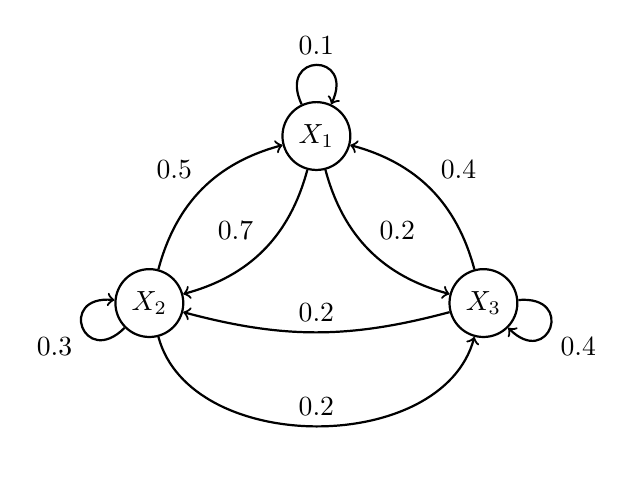
\begin{tikzpicture}[node distance={30mm}, thick, main/.style = {draw, circle}] 
    \node[main] (1) {$X_1$}; 
    \node[main] (2) [below left of=1] {$X_2$}; 
    \node[main] (3) [below right of=1] {$X_3$};
    \draw[->] (1) to [out=115,in=65,looseness=5] node[midway, above, pos=0.5] {0.1} (1);
    \draw[->] (1) to [out=-105,in=15,looseness=1] node[midway, above left, pos=0.5] {0.7} (2);
    \draw[->] (1) to [out=-75,in=165,looseness=1] node[midway, above right, pos=0.5] {0.2} (3);
    \draw[->] (2) to [out=75,in=195,looseness=1] node[midway, above left, pos=0.5] {0.5} (1);
    \draw[->] (2) to [out=225,in=175,looseness=5] node[midway, below left, pos=0.5] {0.3} (2);
    \draw[->] (2) to [out=285,in=255,looseness=1] node[midway, above, pos=0.5] {0.2} (3);
    \draw[->] (3) to [out=105,in=-15,looseness=1] node[midway, above right, pos=0.5] {0.4} (1);
    \draw[->] (3) to [out=195,in=-15,looseness=1] node[midway, above, pos=0.5] {0.2} (2);
    \draw[->] (3) to [out=5,in=-45,looseness=5] node[midway, below right, pos=0.5] {0.4} (3);
    \label{fig:sampleChain1}
    \end{tikzpicture}
    \caption{Ejemplo de una cadena de Markov} 
    \label{fig:sampleChain1}
    \end{figure}
    
    Internamente, las cadenas de Markov se suelen representar con matrices de transición, tales como la de la tabla \ref{tab:sampleChainMatrix}

    \begin{table}
	\centering
	\begin{tabular}{c|c|c|c}
		\textbf{} & \textbf{$X_1$} & \textbf{$X_2$} & \textbf{$X_3$}\\
		\hline
		\textbf{$X_1$} & 0.1 & 0.7 & 0.8\\
		\hline
		\textbf{$X_2$} & 0.5 & 0.3 & 0.2\\
		\hline
		\textbf{$X_3$} & 0.4 & 0.2 & 0.4\\
	\end{tabular}
	\caption{Ejemplo de una matriz de transición}
	\label{tab:sampleChainMatrix}
    \end{table}
    
    \subsection{Entrenamiento de las Cadenas de Markov}
    \label{subsec:entrenamientoCadenasMarkov}
    Una ventaja de las cadenas de Markov es su fácil entrenamiento. Una vez tenemos nuestro dataset limpio y normalizado (como se explica en \ref{sec:dataset}) podemos recorrerlo para construir la matriz de transición.

    En nuestro caso, cargamos todas las secuencias de notas del dataset, descartamos las notas que no tienen otra a continuación (serían las que se encuentran al final de la melodía) y rellenamos una tabla de ocurrencias con cada vez que una nota específica se encuentra después de otra.

    Por ejemplo, si hubieran sólo 4 notas (cabe destacar que las notas se encuentran en notación \textit{pitch\_duración}, dicha notación se explica en \ref{subsub:representacion-pitch_duracion}) podría quedar la matriz de ocurrencias dada en la tabla \ref{tab:sampleOcurrenceMatrix} tras recorrer todo el dataset.

    \begin{table}
	\centering
	\begin{tabular}{c|c|c|c|c}
		\textbf{} & \textbf{$60\_2$} & \textbf{$64\_1$} &         
            \textbf{$65\_2$} &     \textbf{$67\_1$}\\
		\hline
		\textbf{$60\_2$} & 238 & 119 & 280 & 63\\
		\hline
		\textbf{$64\_1$} & 120 & 50 & 185 & 145\\
		\hline
		\textbf{$65\_2$} & 117 & 108 & 15 & 60\\
		\hline
		\textbf{$67\_1$} & 120 & 20 & 36 & 24\\
	\end{tabular}
	\caption{Ejemplo de matriz de ocurrencia}
	\label{tab:sampleOcurrenceMatrix}
    \end{table}

    Posteriormente sumamos cada fila y convertimos a probabilidades cada entrada de la tabla dividiendo entre la suma de su fila. Con esto obtenemos una matriz de transición como la de la tabla \ref{tab:sampleTransitionMatrix}.

    \begin{table}
	\centering
	\begin{tabular}{c|c|c|c|c}
		\textbf{} & \textbf{$60\_2$} & \textbf{$64\_1$} &         
            \textbf{$65\_2$} &     \textbf{$67\_1$}\\
		\hline
		\textbf{$60\_2$} & 0.34 & 0.17 & 0.4 & 0.09\\
		\hline
		\textbf{$64\_1$} & 0.24 & 0.1 & 0.37 & 0.29\\
		\hline
		\textbf{$65\_2$} & 0.39 & 0.36 & 0.05 & 0.2\\
		\hline
		\textbf{$67\_1$} & 0.60 & 0.1 & 0.18 & 0.12\\
	\end{tabular}
	\caption{Ejemplo de matriz de transición calculada a partir de la matriz de ocurrencia}
	\label{tab:sampleTransitionMatrix}
    \end{table}

    Con la matriz de transición ya podríamos ejecutar la cadena de markov durante N iteraciones para obtener una melodía. En nuestro caso utilizamos la librería de Python PYDTMC, que proporciona modelos de markov ya implementados (para más información sobre dicha librería consultar \cite{PYDTMC}). Con esta librería podemos crear una cadena de Markov a partir de la matriz de transición y poder guardarla a archivo, ejecutar o bien N pasos o paso a paso y dibujarla con matplotlib.
    
    La representación gráfica de la cadena se puede ver en la figura \ref{fig:sampleNotesChain}.

    \begin{figure}
    \centering
    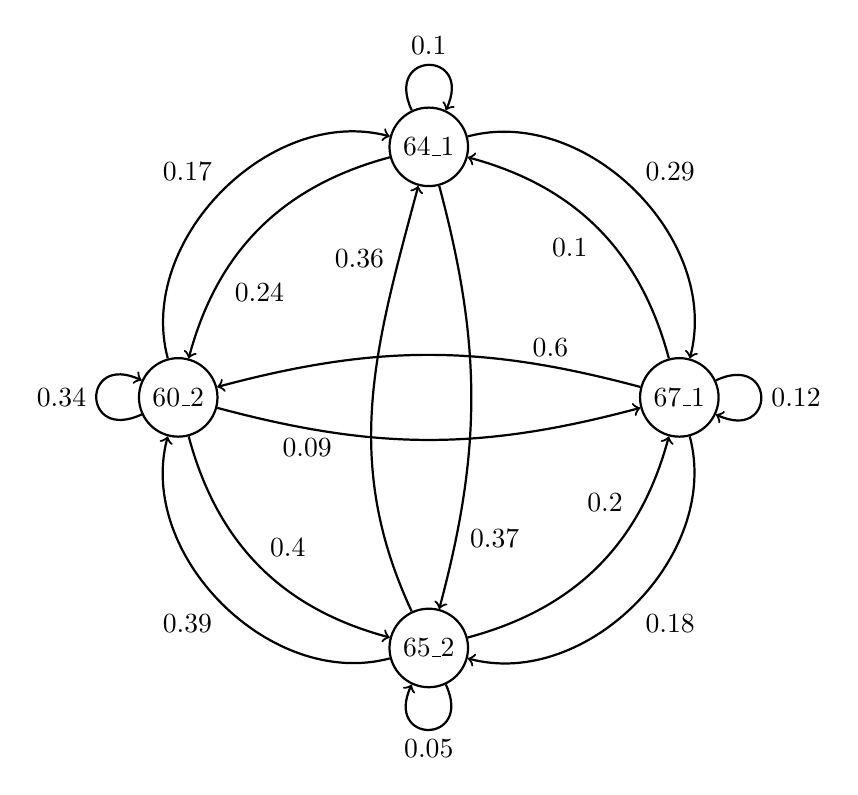
\begin{tikzpicture}[node distance={45mm}, thick, main/.style = {draw, circle}] 
    \node[main] (1) {$60\_2$}; 
    \node[main] (2) [above right of=1] {$64\_1$}; 
    \node[main] (3) [below right of=1] {$65\_2$};
    \node[main] (4) [below right of=2] {$67\_1$};
    \draw[->] (1) to [out=205,in=155,looseness=5] node[midway, left, pos=0.5] {0.34} (1);
    \draw[->] (1) to [out=105,in=165,looseness=1] node[midway, above left, pos=0.5] {0.17} (2);
    \draw[->] (1) to [out=-75,in=-195,looseness=1] node[midway, above right, pos=0.5] {0.4} (3);
    \draw[->] (1) to [out=-15,in=195,looseness=1] node[midway, below , pos=0.2] {0.09} (4);
    \draw[->] (2) to [out=195,in=75,looseness=1] node[midway, below right, pos=0.7] {0.24} (1);
    \draw[->] (2) to [out=115,in=65,looseness=5] node[midway, above, pos=0.5] {0.1} (2);
    \draw[->] (2) to [out=-75,in=75,looseness=1] node[midway, below right, pos=0.8] {0.37} (3);
    \draw[->] (2) to [out=15,in=75,looseness=1] node[midway, above right, pos=0.5] {0.29} (4);
    \draw[->] (3) to [out=195,in=255,looseness=1] node[midway, below left, pos=0.5] {0.39} (1);
    \draw[->] (3) to [out=115,in=255,looseness=1] node[midway, above left, pos=0.8] {0.36} (2);
    \draw[->] (3) to [out=295,in=245,looseness=5] node[midway, below, pos=0.5] {0.05} (3);
    \draw[->] (3) to [out=15,in=255,looseness=1] node[midway, above left, pos=0.7] {0.2} (4);
    \draw[->] (4) to [out=165,in=15,looseness=1] node[midway, above, pos=0.2] {0.6} (1);
    \draw[->] (4) to [out=105,in=-15,looseness=1] node[midway, below left, pos=0.5] {0.1} (2);
    \draw[->] (4) to [out=-75,in=-15,looseness=1] node[midway, below right, pos=0.5] {0.18} (3);
    \draw[->] (4) to [out=25,in=-25,looseness=5] node[midway, right, pos=0.5] {0.12} (4);
    \end{tikzpicture}
    \caption{Representación visual de la cadena obtenida a partir de la matriz de transición} 
    \label{fig:sampleNotesChain}
    \end{figure}

    \subsection{Generar melodías con Cadenas de Markov}
    \label{subsec:generarCadenasMarkov}
    Para crear melodías, podemos realizar el número de iteraciones que queramos sobre la cadena para crear una melodía de la longitud deseada, el acercamiento más simple sería generar N notas. 
    
    En nuestro generador (definido en markovGenerator.py) se puede especificar el número de steps deseado y se generarán iteraciones suficientes hasta llegar al límite. Al ejecutar comenzamos siempre en "C4\_2", por conveniencia.

    El modelo nos construye una melodía que posee cierta coherencia debido al entrenamiento, pero al existir aleatoriedad, es un modelo que no es determinista, por lo que cada melodía será distinta.

    \subsection{Puntos fuertes y débiles de la generación de melodías con Cadenas de Markov}
    \label{subsec:ventajasYDesventajasMarkov}
    Las cadenas de Markov resultan muy potentes como primer acercamiento, pues son un modelo simple y fácil de entender. El entrenamiento es sencillo y su ejecución una vez entrenada es prácticamente instantánea.

    Sin embargo, tienen algunas desventajas. Primero, hablando de rendimiento y escalabilidad, cada nodo de la cadena tiene que representar una nota con duración como mínimo, por lo que en la práctica se crea una cadena inmensa aunque limitemos a 2 octavas el posible rango melódico. Además, aunque la ejecución de pasos en la cadena sea instantáneo, el coste de cargarla y guardarla a archivo es muy grande, pudiendo tardar más de medio minuto.

    Además, desde el punto de vista musical, no proporcionan una melodía muy rica, ya que dependen completamente de la probabilística, las melodías generadas no tendrán una coherencia aparente. Aunque ese punto no resulta muy crítico para nuestro trabajo por el resto de etapas que realizamos, es conveniente obtener una melodía lo más agradable posible.

    Por estos inconvenientes, resulta interesante explorar otros modelos.

\section{Redes Neruonales Recurrentes}
\label{sec:RNR}

\section{Magenta}
\label{sec:magenta}
    \subsection{¿Qué es Magenta?}
    \label{subsec:definicionMagenta}
    Magenta es un proyecto de investigación propiedad de Google, compuesto por varios modelos de machine learning. Estos modelos están entrenados para generar tanto música como dibujos.

    Particularmente, los modelos entrenados con música pueden realizar varias funcionalidades. Existen modelos que generan melodías, modelos que continúan una melodía dada, generar baterías, autoencoders que permiten humanizar baterías, armonizar una melodía dada... Podemos encontrar estos modelos y más en el repositorio de Magenta (\cite{MagentaRepo}) o en su web (\cite{MagentaWeb}).

    Magenta contiene además un plugin para la DAW Ableton llamado Magenta Studio (\cite{MagentaStudio}). Dicho plugin fue además porteado a aplicación de escritorio para Windows. En este plugin encontramos varios programas que desmuestran la funcionalidad de Magenta, como: Generate, que genera melodías de 4 compases; Continue, que continúa una melodía de entrada un número N de compases; Drumify, que crea una base de batería dado un ritmo de input; Interpolate, que crea una melodía o base de tambor combinando 2 de entrada; y finalmente Groove, que humaniza una base de tambor para que suene como una persona.
    
    \subsection{Paquete de Magenta para Python}
    \label{subsec:magentaPython}
    Existe un paquete de Magenta para Python, que puede ejecutar todos los modelos preentrenados.

    Dicho paquete tiene instrucciones de instalación para sistemas Linux y MacOS (consultar \cite{MagentaRepo}), sin embargo, a día de hoy no parece tener una versión compatible con Windows, por lo que no podemos utilizarlo en nuestra aplicación.

    \subsection{Paquete de Magenta para JavaScript}
    \label{subsec:magentaJS}
    Magenta tiene también una versión para JavaScript, que se ejecuta sobre TensorFlowJS. Dicha versión es análoga a la de Python y permite ejecutar los modelos preentrenados.

    Magenta Studio utiliza esta versión de Magenta, tanto para el plugin de Ableton como en la versión de escritorio, por lo que podemos utilizar esta versión para incluir Magenta en nuestro proyecto.

    \subsection{Magenta en nuestro proyecto}
    \label{subsec:magentaEnNuestroProyecto}
    Para poder comunicar nuestro proyecto de Python con Magenta utilizamos el módulo de Python \textit{subprocess}.

    Podemos tener diversos scripts de NodeJS que son ejecutados por un script Python y se comunican por los argumentos del proceso y la salida estándar de este. 

    Actualmente tenemos 2 scripts, uno dedicado a generar melodías (magentaGenerator.js) y otro dedicado a continuar melodías ya creadas (magentaContinue.js).

    En la aplicación tenemos la posibilidad de generar melodías con Magenta, requiriendo una conexión a internet para descargar y ejecutar el modelo preentrenado.

    \subsection{Ventajas y desventajas de la generación con Magenta}
    \label{ventajasYDesventajasMagenta}
    Generar melodías con Magenta nos aporta varias ventajas respecto a modelos anteriores.

    Son modelos entrenados con una gran cantidad de datasets y que utilizan técnicas avanzadas de machine learning, por tanto, la generación de melodías es bastantes más rica que en otros modelos propios y estas poseen más coherencia interna.

    Además, el \textit{continue} nos permite alargar melodías y mantenerlas coherentes para poder trabajar con ellas posteriormente.

    Sin embargo, como desventaja principal tenemos la necesidad de una conexión a internet para poder utilizar el modelo, así como el tiempo que tarda el modelo en inicializar, sobre todo al tener que manejar subprocesos.

    Este modelo de generación nos aporta bastantes ventajas, pero es necesario mantener algún modelo que se pueda ejecutar de forma local y no dependa de módulos que a futuro puedan ser descontinuados.
\chapter{Armonización}
\label{cap:armonizacion}



\section{¿Qué es armonizar?}
    \subsection{Pequeña introducción a la música}\label{sec:arm:armonia}

        Para entender lo explicado en posteriores secciones primero se hará en pequeño resumen de teoría musical. Vamos a definir la música como un conjunto de sonidos de duración variable organizados en el tiempo y que tienen cierto sentido estético, ya que pretenden transmitir emociones, ideas o belleza.

        Por lo tanto y, sintetizando al máximo, a nivel simbólico una canción la definen dos elementos: un conjunto de sonidos y un ritmo, es decir, la duración y el instante de tiempo en el que empieza cada sonido de ese conjunto. Nos centraremos por ahora en el primer elemento, ¿qué conjunto de sonidos se puede utilizar para componer una canción?
        Técnicamente cualquiera, al tratarse de una disciplina artística existe libre albedrío para realizar una composición. 

        \label{arm:notas_musicales}
        Sin embargo, nos centraremos en el estándar occidental, utilizado prácticamente en todas canciones que escuchamos diariamente, en el que los sonidos se dividen en conjuntos de 12 notas musicales, cada una con un nombre diferente, difiniendo nota musical como un símbolo que representa una frecuencia determinada. Para entender de dónde viene esta división utilizaremos como base la nota A4 (La4), con una frecuencia de 440Hz y duplicaremos su frecuencia a 880Hz, obteniendo así A5 (La5). Estas dos notas comparten nombre, ya que si las escucháramos nos sonarían muy familiares entre sí. Esto tiene una explicación física: al reproducir esa frecuencia (frotando una cuerda, elevando una columna de aire...), no solo se genera la frecuencia fundamental, sino que también se producen armónicos, que son múltiplos enteros de la frecuencia fundamental. Se llama octava a la distancia que separa una frecuencia de su duplicación, esto explica ahora los número escritos al lado de cada nota musical: A3 = 220Hz, A4 = 440Hz, A5 = 880Hz. Sabiendo esto se decidió entonces dividir la octava en 12 notas musicales, perceptualmente equidistantes, la cual difiere con una equidistancia a nivel de frecuencia, debido a la naturaleza exponencial de las frecuencias. Es la llamada afinación temperada:

\begin{table}[h]
    \centering
    \begin{tabular}{c|c}
        \textbf{Nota Musical} & \textbf{Frecuencia (Hz)} \\
        \hline
        A4 & 440.00 \\
        A\#4 & 466.16 \\
        B4 & 493.88 \\
        C5 & 523.25 \\
        C\#5 & 554.37 \\
        D5 & 587.33 \\
        D\#5 & 622.25 \\
        E5 & 659.26 \\
        F5 & 698.46 \\
        F\#5 & 739.99 \\
        G5 & 783.99 \\
        G\#5 & 830.61 \\
        A5 & 880.00 \\
    \end{tabular}
    \caption{Tabla de Afinación Temperada de 12 Notas de A4 a A5}
    \label{tab:temperedTuningTable_A4_A5}
\end{table}

        Sacamos como conclusión que el conjunto de sonidos utilizados está comprendido por las 12 notas musicales, cada una puediéndose encontrar en una octava distinta. Hemos cambiado ligeramente la definición simbólica de canción entonces, pasando esta a estar compuestas por un ritmo y un conjunto de notas musicales (en vez de un conjunto de sonidos).  

        Así mismo, y entrando en otra capa de profundidad, ese conjunto de notas musicales que conformar una canción puede ser dividida en dos partes:

        \begin{enumerate}
            \item[\textbullet] \textbf{Melodía}: línea principal o motivo musical que guía la dirección y el desarrollo de una pieza musical. Parte más reconocible de una canción. En una composición musical es la que generalmente se canta o se toca de manera prominente.
            \item[\textbullet] \textbf{Armonía}: combinación simultánea de dos o más notas que se escuchan juntas y que suenan de manera agradable o consonante. La armonía proporciona un acompañamiento sonoro a la melodía principal y contribuye a enriquecer la textura musical. Se compone de acordes, que son grupos de notas tocadas simultáneamente.

        \end{enumerate}

    \subsection{Pequeña introducción a la armonía}

        Como se acaba de explicar, la armonía se define como la combinación y disposición de notas musicales que suenan de manera agradable y coherente entre sí. Para entender tanto la armonía, como los algoritmos que se quieren mostrar en este apartado del TFG, es necesario interiorizar los siguientes conceptos, que se intentarán explicar de la manera más resumida posible. Cabe recalcar que la explicación se realiza en el contexto de la armonía moderna, la cual difiere en algunos puntos de la clásica, sin embargo, al tratarse de una introducción, la mayoría de conceptos que van a ser mostrados se comparten entre ambas doctrinas. 

\begin{figure}[h]
    \centering
    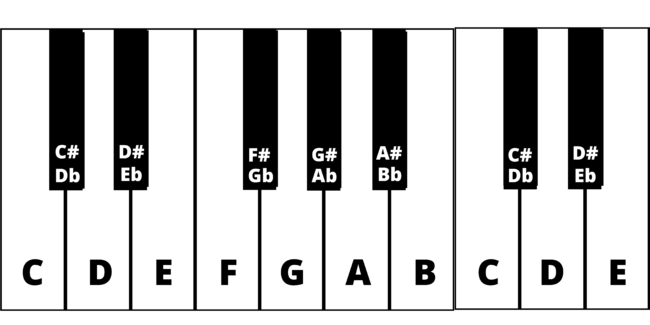
\includegraphics[width = 0.5\textwidth]{Imagenes/Bitmap/piano.png}
    \caption{Notas en el Piano}
    \label{fig:pianoImage}
\end{figure}

        \subsubsection{Intervalos}\label{sec:arm:intervalos}

        Un intervalo es la distancia que existe entre dos notas. Un semitono es la distancia mínima que puede existir entre dos notas. Un tono es igual a dos semitonos. Por ejemplo, en la figura \ref{fig:pianoImage} se puede observar que la distancia entre el primer C y el primer E es de 4 semitonos (las teclas negras también cuentan como notas musicales aunque tengan nombres un poco especiales). Podemos encontrar esa distancia mínima de un semitono entre C y C\# o entre E y F, por ejemplo. Dependiendo del número de semitonos que tenga un intervalo, este tendrá un nombre y simbología diferente (también llamada grado en ciertos contextos que veremos posteriormente):

\begin{table}[h]
    \centering
    \begin{tabular}{c|c|c}
        \textbf{Símbolo (grado)} & \textbf{Nombre} & \textbf{Nº Semitonos} \\
        \hline
        1 (T) & Tónica & 0 \\
        b2 & Segunda menor & 1 \\
        2 & Segunda Mayor & 2 \\
        b3 & Tercera menor & 3 \\
        3 & Tercera Mayor & 4 \\
        4 & Cuarta Justa & 5 \\
        \#4 & Cuarta Aumentada & 6 \\
        5b & Quinta disminuida & 6 \\
        5 & Quinta Justa & 7 \\
        b6 & Sexta menor & 8 \\
        6 & Sexta Mayor & 9 \\
        b7 & Séptima menor & 10 \\
        7 & Séptima Mayor & 11 \\
        8 & Octava & 12 \\
    \end{tabular}
    \caption{Tabla de Intervalos}
    \label{tab:tabla_intervalos}
\end{table}

    Al observar la tabla se puede deducir por contexto que el símbolo 'b' (bemol) reduce en uno el número de semitonos del grado original, así como el símbolo '\#' (sostenido) los aumenta en uno. Por ejemplo, \#6 sería equivalente a una séptima menor (b7), con 10 semitonos ambos. Así mismo estos símbolos se pueden apilar, por ejemplo, bb7 sería equivalente a una sexta Mayor (6), con 9 semitonos ambos.

    Con la información de esta tabla, ya podríamos entender afirmaciones tales como 'la quinta Justa de C es G' o 'la tercera Mayor de B es D\#', por ejemplo, si nos ponemos a contar los semitonos más detenidamente.

    Cabe recalcar que, evidentemente, existen intervalos que se salen de la octava, con más de 12 semitonos. Algunos no muy lejanos tienen incluso nombre propio, por ejemplo, una novena Mayor (9), de 14 semitonos. A pesar de ello, lo que se hará en estos casos es interpretar ese intervalo como su relativo si la nota estuviese en el 'mismo rango' que la tónica (nota desde la cual se mide el intervalo). Así, una novena Mayor sería equivalente a una segunda Mayor, de 2 semitonos y un intervalo de 42 semitonos será interpretado como una quinta disminuida (42 mod 12 = 6 semitonos), por ejemplo. De hecho, siguiendo esta definición, el propio intervalo de octava es redundante, ya que esta es equivalente a la tónica y cumple la misma función (12 mod 12 = 0 semitonos). Por ejemplo, la octava de C4 es C5. Por ello, el intervalo de octava también se debería quitar de la lista.

    \subsubsection{Escalas}\label{sec:arm:escalas}

    Se define escala como conjunto de 2 a 12 intervalos o grados ascencentes cuyo primer intervalo es siempre la tónica. Tradicionalmente, la mayoría de escalas están formadas por 7 grados, las más utilizadas en la música que escuchamos hoy en día son la Mayor y la menor.

\begin{table}[h]
    \centering
    \begin{tabular}{c|c|c|c|c|c|c|c}
        \textbf{Escala Mayor} & 1 (T) & 2 & 3 & 4 & 5 & 6 & 7 \\
        \hline
        \hline
        \textbf{Escala menor} & 1 (T) & 2 & b3 & 4 & 5 & b6 & b7 \\
    \end{tabular}
    \caption{Escalas Mayor y menor}
    \label{tab:escalas}
\end{table}

    Este conjunto de intervalos representa una especie de esqueleto, un molde con el cual se puede crear una sucesión de notas musicales si se establece como tónica cualquiera de las 12 notas existentes. Aquí uno cuantos  ejemplos, utilizando como tónicas C, D y Bb:

\begin{table}[h]
    \centering
    \begin{tabular}{c|c|c|c|c|c|c|c}
        \textbf{C Mayor} & C (T) & D & E & F & G & A & B \\
        \hline
        \textbf{D Mayor} & D (T) & E & F\# & G & A & B & C\# \\
        \hline
        \textbf{Bb Mayor} & Bb (T) & C & D & Eb & F & G & A \\
        \hline
        \hline
        \textbf{C menor} & C (T) & D & Eb & F & G & Ab & Bb \\
        \hline
        \textbf{D menor} & D (T) & E & F & G & A & Bb & C \\
        \hline
        \textbf{Bb menor} & Bb (T) & C & Db & Eb & F & Gb & Ab \\
    \end{tabular}
    \caption{Escalas y Tónicas}
    \label{tab:escalas_tonicas}
\end{table}

    Para poner un poco más en contexto decir que, a parte de estas dos escalas, existen muchas otras más que se utilizan regularmente a la hora de componer música. Incluso existen compositores más vanguardistas que inventan nuevos conjuntos de grados, experimentando con nuevas formas de escribir música. Elgunos ejemplos: 

\begin{table}[h]
    \centering
    \begin{tabular}{c|c|c|c|c|c|c|c}       
        \textbf{pentatónica Mayor} & 1 (T) & 2 & 3 & 5 & \multicolumn{1}{c}{6} \\
        \hline
        \textbf{pentatónica menor} & 1 (T) & b3 & 4 & 5 & \multicolumn{1}{c}{b6} \\
        \hline
        \textbf{hexatónica} & 1 (T) & 2 & 3 & \#4 & \#5 & \multicolumn{1}{c}{\#6}  \\
        \hline
        \textbf{frigia} & 1 (T) & b2 & b3 & 4 & 5 & b6 & b7 \\
        \hline
        \textbf{mixolidia} & 1 (T) & 2 & 3 & 4 & 5 & 6 & b7 \\
        \hline
        \textbf{menor armónica} & 1 (T) & 2 & b3 & 4 & 5 & b6 & 7 \\      
    \end{tabular}
    \caption{Otras Escalas}
    \label{tab:otras_escalas}
\end{table}

    \subsubsection{Acordes}\label{sec:arm:acordes}

    Aunque no todo el mundo estaría de acuerdo con esta definición, vamos a decir que un acorde es un conjunto de dos o más notas tocadas de forma simultánea. La definición es en cierta medida similar a la de una escala, ya que un acorde no deja de ser un conjunto de intervalos ascendentes, en el que el primero es simpre la tónica del acorde. También se cumple esa propiedad de 'molde' a la hora de establecer una nota musical como tónica del acorde. Los acordes más comunes están formados por tres notas (tríadas) y dependiendo del conjunto de intervalos se pueden conseguir diferentes sonoridades:

\begin{table}[h]
    \centering
    \begin{tabular}{c|c|c|c|c}       
        \textbf{Nombre} & \textbf{Símbolo} & \multicolumn{3}{c}{\textbf{Intervalos}} \\
        \hline
        \hline
        \textbf{Acorde Mayor} & & 1 (T) & 3 & 5 \\
        \hline
        \textbf{Acorde menor} & - & 1 (T) & b3 & 5 \\
        \hline
        \textbf{Acorde Aumentado} & + & 1 (T) & 3 & \#5 \\
        \hline
        \textbf{Acorde disminuido} & -b5 & 1 (T) & b3 & b5 \\
    \end{tabular}
    \caption{tríadas}
    \label{tab:triads}
\end{table}

\begin{table}[h]
    \centering
    \begin{tabular}{c|c|c|c|c}       
        \textbf{Nombre} & \textbf{Símbolo} & \multicolumn{3}{c}{\textbf{Notas}} \\
        \hline
        \hline
        \textbf{C Mayor} & C & C (T) & E & G \\
        \hline
        \textbf{C menor} & C- & C (T) & Eb & G \\
        \hline
        \textbf{C Aumentado} & C+ & C (T) & E & G\# \\
        \hline
        \textbf{C disminuido} & C-b5 & C (T) & Eb & Gb \\
    \end{tabular}
    \caption{tríadas en C}
    \label{tab:triadsC}
\end{table}

    \label{arm:armonia_escala}
    Se define como armonía de una escala el conjunto de acordes que se pueden formar utilizando únicamente las notas (o intervalos) de la escala. Esto puede chocar con la definición de acorde, ya que, como tal, puede haber miles de tipos de acordes diferentes si atendemos a toda la combinatoria, así que, por ahora, solo tendremos en cuenta los tipos de acordes definidos anteriormente, es decir, acordes mayores, menores, aumentados y disminuidos. Este concepto es más difícil de deducir y explicar, así que recomiendo la visualización de \href{https://www.youtube.com/watch?v=dMwVB3BWcjI}{este vídeo} en el que el autor encuentra la armonía de la escala C Mayor y pasa el resultado a grados, además de repasar otros conceptos vistos por encima anteriormente. Se obtiene el siguiente resultado:

\begin{table}[h]
    \centering
    \begin{tabular}{c|c||c|c}
        \textbf{Grado} & \textbf{Acorde} & \textbf{Nota} & \textbf{Acorde} \\
        \hline
        1 (T) &  & C (T) & C \\
        2 & - & D & D- \\
        3 & - & E & E- \\
        4 &  & F & F \\
        5 &  & G & G \\
        6 & - & A & A- \\
        7 & -b5 & B & B-b5 \\
    \end{tabular}
    \caption{Escala Mayor en Grados y en C}
    \label{tab:grados_C}
\end{table}

    Como se puede observar, en la escala Mayor se forma una tríada mayor a partir de los grados 1, 4 y 5, una menor a partir de los grados 2, 3 y 6, una disminuida a partir del grado 7 y no existe ningún grado del cual se forme una tríada aumentada. Esto significa que sea cual sea la tónica de una escala, en este caso, la escala Mayor, los acordes correspondientes a cada grado serán siempre del mismo tipo. Por lo tanto, si se quiere deducir la armonía de una escala diferente, por ejemplo, la escala menor, los acordes correspondientes a cada grado serán distintos a los de la escala Mayor, pero serán del mismo tipo si se varía la tónica. Además, el hecho de que solo se forme un acorde por cada grado es debido a una particularidad propia de la escala Mayor y a que hemos escogido un número muy reducido de acordes. Vamos a tener en cuenta ahora el siguiente grupo de acordes de cuatro notas (cuatríadas), que se sumarán al anterior grupo:

\begin{table}[h]
    \centering
    \begin{tabular}{c|c|c|c|c|c}       
        \textbf{Nombre} & \textbf{Símbolo} & \multicolumn{4}{c}{\textbf{Intervalos}} \\
        \hline
        \hline
        \textbf{Acorde Mayor séptima} & maj7 & 1 (T) & 3 & 5 & 7\\
        \hline
        \textbf{Acorde de Dominante} & 7 & 1 (T) & 3 & 5 & b7\\
        \hline
        \textbf{Acorde menor séptima} & -7 & 1 (T) & b3 & 5 & b7 \\
        \hline
        \textbf{Acorde semidisminuido} & -7b5 & 1 (T) & b3 & b5 & b7 \\
        \hline
        \textbf{Acorde disminuido} & º & 1 (T) & b3 & b5 & bb7 \\
    \end{tabular}
    \caption{Cuatríadas}
    \label{tab:cuatriads}
\end{table}

    A continuación un par de ejemplos que evidencian el anterior párrafo: (Tabla \ref{tab:comparativa_scalas})

\begin{table}[h]
    \centering
    \begin{tabular}{c|c|c||c|c|c||c|c|c}
        \multicolumn{3}{c}{} & \multicolumn{3}{c}{\textbf{Escala Mayor}}  \\
        \hline  
        \multicolumn{1}{c|}{\textbf{Grados}} & \multicolumn{2}{c||}{\textbf{Acordes}} & \multicolumn{1}{c|}{\textbf{Notas}} & \multicolumn{2}{c||}{\textbf{Acordes}} & \multicolumn{1}{c|}{\textbf{Notas}} & \multicolumn{2}{c}{\textbf{Acordes}} \\
           \hline
    1 (T) &     & maj7 & C (T) & C    & Cmaj7 & D (T)   & D      & Dmaj7   \\
        2 & -   & -7   &    D  & D-   & D-7   &    E    & E-     & E-7     \\
        3 & -   & -7   &    E  & E-   & E-7   &    F\#  & F\#-   & F\#-7   \\
        4 &     & maj7 &    F  & F    & Fmaj7 &    G    & G      & Gmaj7   \\
        5 &     & 7    &    G  & G    & G7    &    A    & A      & A7      \\
        6 & -   & -7   &    A  & A-   & A-7   &    B    & B-     & B-7     \\
        7 & -b5 & -7b5 &    B  & B-b5 & B-7b5 &    C\#  & C\#-b5 & C\#-7b5 \\
        \hline
        \multicolumn{3}{c}{} & \multicolumn{3}{c}{\textbf{Escala menor}}  \\
        \hline  
        \multicolumn{1}{c|}{\textbf{Grados}} & \multicolumn{2}{c||}{\textbf{Acordes}} & \multicolumn{1}{c|}{\textbf{Notas}} & \multicolumn{2}{c||}{\textbf{Acordes}} & \multicolumn{1}{c|}{\textbf{Notas}} & \multicolumn{2}{c}{\textbf{Acordes}} \\
           \hline 
    1 (T)  & -   & -7   & C (T)  & C-    & C-7    & D (T) & D-   & D-7    \\
        2  & -b5 & -7b5 &    D   & Db-b5 & Db-7b5 &    E  & E-b5 & E-7b5  \\
        b3 &     & maj7 &    Eb  & E     & Emaj7  &    F  & F    & Fmaj7  \\
        4  & -   & -7   &    F   & F-    & F-7    &    G  & G-   & G-7    \\
        5  & -   & -7   &    G   & G-    & G-7    &    A  & A-   & A-7    \\
        b6 &     & maj7 &    Ab  & Ab    & Abmaj7 &    Bb & Bb   & Bbmaj7 \\
        b7 &     & 7    &    Bb  & Bb    & Bb7    &    C  & C    & C7     \\

    \end{tabular}
    \caption{Comparativa entre Escalas (Mayor y menor) y Tónicas (C y D)}
    \label{tab:comparativa_scalas}
\end{table}
    

    Todo lo mostrado hasta ahora forma parte de las bases de composición musical. Básicamente escoger una escala y una tónica, y utilizar todo el conjunto de notas y acordes que se forman a partir de estas para crear una melodía y una armonía (un acompañamiento). Sin embargo, esto es solo la punta del iceberg, ya que si se prfundiza, se podrán descubrir otros conceptos, como la modulación (cambio de tonalidad), el uso de acordes y notas de otras escalas, la libertad para salirse de las restricciones de la escala establecida, etc. 

\subsection{Cuestión a resolver}
\label{sec:arm:cuestion}      

    Una vez que se conoce todo este contexto ya se puede presentar el problema que se pretende abordar en esta sección o módulo de la aplicación: dada una melodía cualquiera, encontrar la armonía que mejor se adapte a esta, es decir, buscar la mejor secuencia de acordes que acompañen y enriquezcan a la melodía. Esta secuencia de acordes sería utilizada por posteriores módulos de la aplicación.

    Cabe dejar claro que, buscar 'la mejor' armonía para una melodía es algo relativo, ya que depende de la subjetividad de cada persona. Así que lo dejaremos en buscar una armonía fuertemente coherente para una melodía dada, que forme parte del espectro de soluciones razonables, ya que, por lo general, una melodía puede ser acompañada por varios conjuntos de acordes distintos.

    También comentar que, al resolver este problema, se estaría construyendo de forma implícita un analizador armónico. Si la entrada a este módulo fuese, en vez de únicamente una melodía, una canción completa, la cual contiene mucha más información, la salida esperada sería la armonía de dicha canción. Esto tiene mucha utilidad, ya que el análisis armónico es fundamental para el estudio en profundidad de una obra. La armonía son los cimientos de una composición musical. 

    \section{Técnicas de armonización utilizadas}

    Antes de empezar con las técnicas de armonización utilizadas, falta un paso previo crucial. Y es la creación de una estructura de clases y métodos que den soporte a todo lo explicado en el apartado \ref{sec:arm:armonia}. Existen clases que abstraen lo que representa una \hyperref[arm:notas_musicales]{\textcolor{blue}{nota musical}}, un \hyperref[sec:arm:intervalos]{\textcolor{blue}{intervalo}}, una \hyperref[sec:arm:escalas]{\textcolor{blue}{escala}} y la \hyperref[arm:armonia_escala]{\textcolor{blue}{armonía de una escala}} tal como se ha explicado. Un \hyperref[sec:arm:acordes]{\textcolor{blue}{acorde}} es respresentado también como una escala. 
    
    También es importante mostrar las respresentaciones que se están utilizando para almacenar una canción (conjunto de notas) en este módulo de la aplicación. Existen métodos para pasar de la primera representación a la segunda:

    \begin{enumerate}
        \item \textbf{Lista de Notas}: es la representación estándar en este módulo de la aplicación. Se almacenan de forma desordenada diccionarios con la siguiente estructura:
        \begin{enumerate}
            \item[\textbullet] \textbf{note}: almacena el pitch MIDI (tono) de la nota. Guardar el pitch MIDI es similar a guardar la nota musical, ya que este almacena de forma implícita el nombre de la nota y su octava. Por ejemplo, calculemos a qué nota le corresponde el pitch 40:
            \begin{enumerate}
                    \item[\(\circ\)] \textbf{Nombre}: 40 mod 12 = 4, según la tabla \ref{tab:nota_pitch} a un 4 le corresponde E.
                    \item[\(\circ\)] \textbf{Octava}: 40 div 12 = 3, está en la tercera octava.
            \end{enumerate}
                       
\begin{table}[htbp]
    \centering
    \begin{tabular}{c|c}
        \textbf{Nombre} & \textbf{Pitch} \\
        \hline
        C & 0 \\
        C\# / Db & 1 \\
        D & 2 \\
        D\# / Eb & 3 \\
        E & 4 \\
        F & 5 \\
        F\# / Gb & 6 \\
        G & 7 \\
        G\# / Ab & 8 \\
        A & 9 \\
        A\# / Bb & 10 \\
        B & 11 \\
    \end{tabular}
    \caption{Relación entre cada Nota Musical y su Pitch en la Primera Octava}
\label{tab:nota_pitch}
\end{table}

        \item[\textbullet] \textbf{start\_time}: tiempo en ticks en el que empieza a sonar una nota desde que empieza la canción en el tick 0.
        \item[\textbullet] \textbf{duration}: tiempo en ticks desde que empieza a sonar la nota hasta que para.
    \end{enumerate}
    \item \textbf{Diccionario de Ticks}: se almacena en cada tick clave el evento que ha ocurrido. Los ticks clave están ordenados de menor a mayor. Como tal, solo existen dos tipos de eventos: 
    \begin{enumerate}
        \item[\textbullet] \textbf{note\_on}
        \item[\textbullet] \textbf{note\_off}
    \end{enumerate}
    A cada evento viene asociado el pitch de la nota afectada. Esto puede suponer, a priori, un inconveniente, ya que, si hay dos notas del mismo pitch superpuestas en el mismo espacio de tiempo, existe una ambigüedad a la hora de saber qué evento \textit{note\_off} le corresponde a cada una. Sin embargo, esta representación se utiliza de forma temporal para facilitar la implementación de ciertos algoritmos a los cuales cuales este inconveniente no les afecta. 
    
\end{enumerate}

    Falta por explicar el concepto de tick. Un tick es la unidad simbólica mínima e indivisible que puede durar una nota. En cada canción (conjunto de notas) se debe definir el número de ticks que dura un pulso. Un pulso también se puede traducir como una negra, un beat o un step. Cuanto mayor sea el número de ticks por pulso, mayor será el número de partes en el que puedes dividir el pulso. Haciendo una analogía con la representación simbólica que se utiliza en las partituras, si los ticks por pulso son iguales a 4, en nuestra canción la semicorchea sería la representación mínima que se podría utilizar, mientras que si fueran igual a 8, la fusa sería la representación mínima (una fusa es la mitad de una semicorchea). De todas formas, lo normal es que los el número de ticks por pulso sea más alto para permitir mayor número de divisiones y combinaciones.

\subsection{Armonización por ventanas} 

    Este fue el primer algoritmo diseñado, el cual escalará y evolucionará en posteriores subapartados. Se basa en una idea, a priori, sencilla: dividir la canción en ventanas. Una ventana es una idea propia, y se define como conjunto de pulsos consecutivos que comprenden las notas que se hallan en dicho segmento. La idea es dividir la canción en ventanas de un determinado número de pulsos y asignar a cada una, es decir, al conjunto de notas que abarca, el acorde que mejor encaje según una heurística.

    Tanto la idea de las ventanas, como la heurística utilizada, están estrechamente relacionadas con cómo funcionan los compases en la música real. En castellano, se define como compás tanto a la fracción que se encuentra al principio de un pentagrama, como a cada uno de los espacios comprendidos entre las líneas (horizontales) divisorias (\ref{fig:sheet4/4}). El denominador de la fracción representa una figura musical, y cada figura musical representa un determinado número de pulsos. En este caso, el denominador es el número 4, que representa una negra, la cual dura un pulso. El numerador nos indica la cantidad de figuras, por ende, la fracción 4/4 nos está diciendo que un compás abarca 4 * 1 = 4 pulsos. 

\begin{figure}[h]
    \begin{center}
        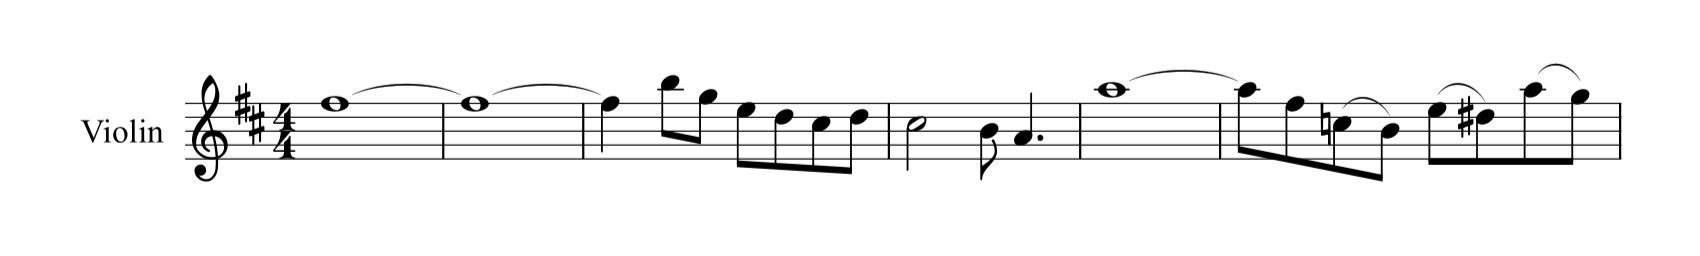
\includegraphics[scale=0.65]{Imagenes/Bitmap/partitura.png}
    \end{center}
    \caption{Partitura en 4/4}
    \label{fig:sheet4/4}
\end{figure}

    Veamos otro ejemplo con el compás 6/8 (\ref{fig:sheet6/8}). El denominador es el número 8, que representa una corchea. La corchea dura medio pulso. El númerador nos indica que en cada compás caben 6 corcheas, es decir 6 * 0.5 = 3 pulsos.

\begin{figure}[h]
    \begin{center}
        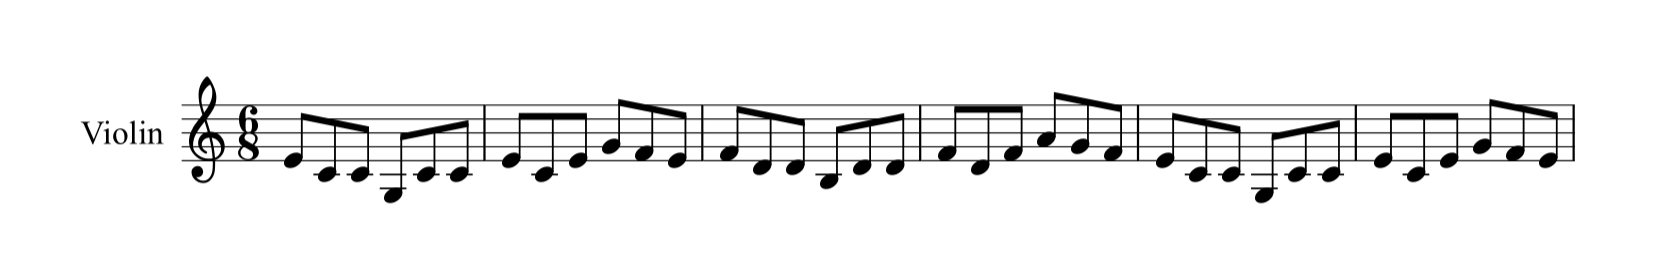
\includegraphics[scale=0.65]{Imagenes/Bitmap/partitura2.png}
    \end{center}
    \caption{Partitura en 6/8}
    \label{fig:sheet6/8}
\end{figure}

    Sabiendo esto, se puede establecer una clara analogía entre los compases y el concepto de ventana. La fracción nos indica el número de pulsos que abarca cada ventana, y las notas encerradas entre las líneas divisorias de cada compás serían las que cada ventana tiene en cuenta para elegir un acorde. 

    La idea es rellenar una lista en la que cada índice represente cada ventana. Dependiendo de cómo de larga sea una canción y cómo de grandes sean las ventanas, el tamaño de la lista variará. Cada ventana contendrá información del peso de todos los acordes que hayan sido valorados para acompañar al conjunto de notas que abarque la ventana. Se elige finalmente el acorde de mayor peso para cada ventana. Si un acorde no aparece en la lista de acordes es porque tiene peso 0, es decir, ni siquiera se ha valorado como candidato para encajar en la ventana. El peso de los acordes se calcula a partir de la heurística que se explicará a continuación.

    Sin embargo, para definir el cómo se va a valorar cada acorde, se ha de elegir antes qué acordes se van a valorar. Primero se debe elegir qué tipo de acordes se quiren detectar. Por ejemplo, el \hyperref[tab:triads]{\textcolor{blue}{conjunto de las cuatro tríadas}} definido anteriormente. Ahora bien, como existen 12 notas musicales, se van a valorar 48 acordes diferentes por cada ventana, y eso solo teniendo encuenta 4 tipos de acordes. Dicha cifra podría escalar. A pesar de esto, el problema está no tanto en el rendimiento, sino en el hecho de que se estarían valorando acordes que contienen notas que no se encuentra en el conjunto de notas de la melodía, es decir, notas fuera de la \hyperref[sec:arm:escalas]{\textcolor{blue}{escala}}, puediendo así aparecer soluciones poco deseadas. Para paliar este problema, se escogerán únicamente acordes cuyo conjunto de notas esté comprendido en la escala que forma el conjunto de notas de la melodía. Es decir, se utilizará la \hyperref[arm:armonia_escala]{\textcolor{blue}{armonía de la escala}} que forma el conjunto de notas de la melodía. Esto mitiga considerablemente el problema, pero no lo llega a solucionar, además de generar otros. Estos problemas se explicarán y se intentarán solucionar en apartados posteriores, por ahora, nos sirve esta solución, ya que esto no es más que una primera versión del algoritmo que se pretende construir.

    A partir de ahora, se trabajará en términos relativos. De hecho, todo lo explicado anteriormente se ha implementado así, aunque en la explicación se haya querido abstraer. Toda la arquitectura del módulo ha sido pensada para trabajar en estos términos relativos. Eso significa que, en vez de con notas musicales, se trabajará con grados e intervalos. Esto se logra estableciendo cualquier nota del conjunto de notas de la melodía como tónica (al menos por ahora; esto podría cambiar en el futuro), la primera mismamente, y relativizando el resto de las notas respecto a esta, es decir, transformando las notas en grados contando el número de semitonos que hay desde la tónica hasta cada nota (\ref{tab:tabla_intervalos}). Véase que, relativizar un conjunto de notas elimina implícitamente la información de la octava. Esto podría suponer un problema, pero lejos de la realidad nos beneficia al tener en cuenta el contexto armónico en el que estamos trabajando. Realmente, no se necesita  información sobre la octava de cada grado, solamente saber a qué grado de la escala pertenece cada nota. También recalcar que el conjunto de grados que se generan a la hora de relativizar todas las notas de la canción formarían ese esqueleto o molde de la escala del que se hablaba en la sección \ref{sec:arm:escalas}. Aunque cueste más de entender, de esta manera se trabaja de forma más sencilla a la hora de ampliar funcionalidades en el módulo. Nótese que también se puede realizar el proceso inverso; es decir, a partir de una tónica y un conjunto de grados, estos se pueden absolutizar para transformarlos en notas musicales.

\subsubsection{Heurística} 

    

    

    


    
\chapter{Generar Percusión por Ordenador}
\label{cap:generacionPercusion}

La percusión\footnote{\url{https://rayrojodrums.com/es/que-son-las-percusiones/}} es una parte fundamental de una canción que aporta ritmo y soporte al resto del arreglo musical. Para la generación de percusión hemos barajado dos opciones, la generación usando \cite{MagentaStudio}(más info en la Sección \ref{sec:magenta}) y la implementación de nuestro propio generador. La opción por la que nos hemos decantado finalmente es la de la generación propia, explicada en la Sección \ref{subsec:generacion-percusion-propia}.


\section{Generación de percusión}
\label{sec:generacion-percusion}

    \subsection{Generación de percusión con Magenta}
    \label{subsec:generacion-percusion-magenta}
    \textit{Drumify} es un programa sencillo dentro de la suite de aplicaciones de Magenta. Su uso es simple pero eficaz: se carga un archivo MIDI (Sección \ref{subsec:que-es-midi}) de una canción, ya sea con acordes o sólo melodía, y devuelve un archivo MIDI con un arreglo batería que funciona para la canción proporcionada. 
    
    Este flujo de trabajo se puede completar usando otra herramienta que nos da Magenta, que en la versión de escritorio llaman \textit{Groove}.
    El \textit{groove} en una canción, en este caso aplicado a la parte de la percusión, es algo así como la sensación de movimiento que genera la canción al escucharla\footnote{\url{https://es.wikipedia.org/wiki/Groove_(musica)}}.
    
    La aplicación \textit{Groove} de Magenta recibe un archivo MIDI, esta vez de percusión, y humananiza las notas, poniendo más velocidad en las notas que suenan en los golpes fuertes del compás, que generalmente serán el bombo y muchas veces la caja, mientras que otros instrumentos como los platillos tendrán menos velocidad. También varía ligeramente la posición de las notas, de forma que no quedan colocadas en el instante de tiempo exacto marcado por el compás, algo que hace que la percusión (y todos los instrumentos en general) suenen bastante robóticos.

    \subsection{Generación de percusión propia}
    \label{subsec:generacion-percusion-propia}
    Una vez vistas las herramientas que nos brinda Magenta para la generación de MIDIs de percusión, llegamos a la conclusión de que era algo que, si bien funcionaba, era demasiado genérico para lo que buscábamos. Por esta razón, no usaremos Magenta en la herramienta.
    
    Hemos implementado nuestro propio generador de percusión, que nos permite trabajar mejor en los estilos que buscábamos, que se presentarán en la Sección \ref{subsubsec:estilos-percusion}. Este generador crea tres archivos MIDI de un compás 4/4 de duración del estilo especificado. A continuación, se especifica su funcionamiento.

    \subsection{¿Cómo enfocamos la percusión?}

    %TODO: working example
    Con el fin de poder programar algún tipo de generador de ritmos de batería, vamos a tratar de simplificar al máximo la forma de crear partes de percusión para una canción.

    El enfoque que vamos a darle es similar al que se explica en el vídeo de YouTube del canal "8-bit Music Theory", (\cite{DrumPartsForNoDrummers})

    Separamos las baterías en tres partes principales:

    \begin{itemize}
        \item \textbf{\textit{Beat}}: Suelen ser notas en los golpes fuertes. Es la parte fundamental del ritmo. Generalmente suele ser el bombo el encargado de esta función.
        \item \textbf{\textit{Engine}}: Son golpes que contrastan con el \textit{beat}. Añaden movimiento al ritmo. Si en el \textit{beat} tenemos un bombo en el \textit{engine} podríamos tener una caja. Pueden ir en los golpes fuertes o en los débiles.
        \item \textbf{\textit{Constant}}: No destaca especialmente pero añade consistencia al ritmo. Esta función suelen desempeñarla los platillos. Suelen ir en los golpes débiles.
    \end{itemize}

    Juntando estas tres partes obtenemos un ritmo de batería base que podemos mantener durante una parte o la totalidad de la canción. Podemos ver un ejemplo de este ritmo en la Figura \ref{fig:ritmo-basico-percusion}, donde la línea de abajo representa el \textit{beat}, en este caso un bombo, la de arriba representa la \textit{constant}, en este caso platillos, y la línea central representa el \textit{engine}, en este caso un golpe de caja.

     \begin{figure}[h]
        \centering
        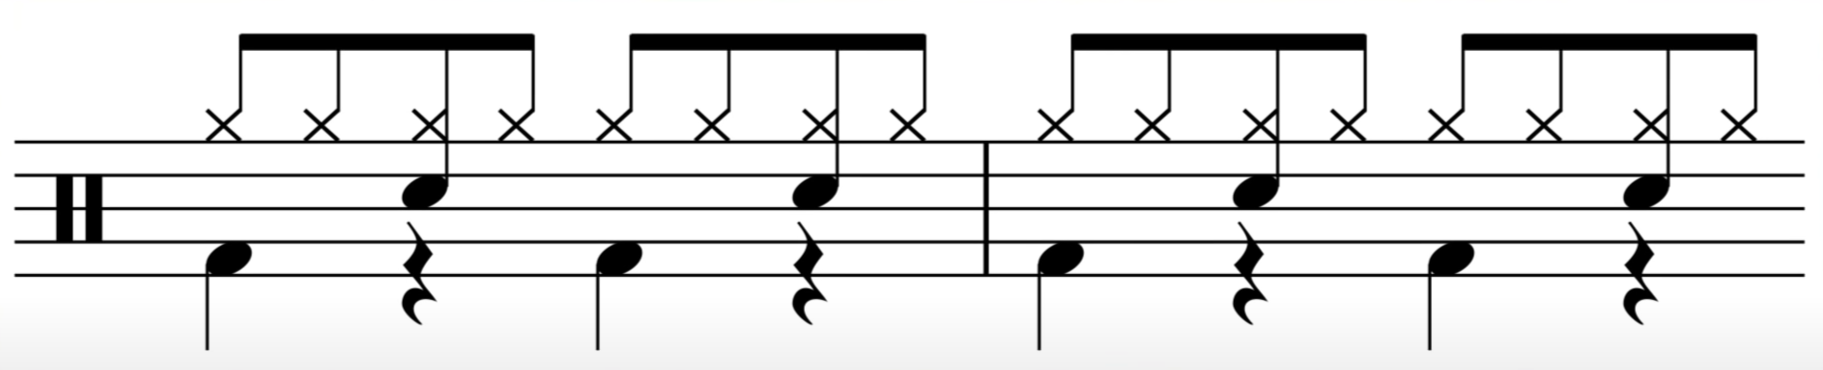
\includegraphics[width = 0.45\textwidth]{Imagenes/Bitmap/BateriaBasico.png}
        \caption{Ritmo básico de percusión.}
        \label{fig:ritmo-basico-percusion}
    \end{figure}

    %TODO: referenciar esta imagen
    \begin{figure}[h]
        \centering
        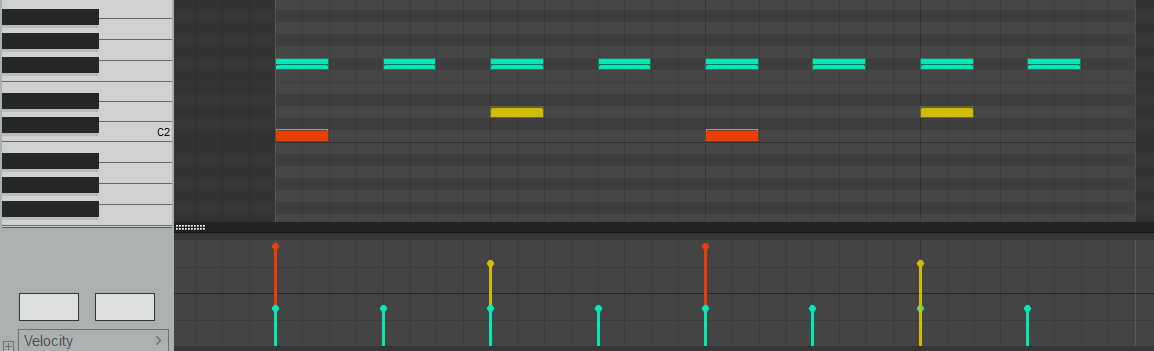
\includegraphics[width = 0.5\textwidth]{Imagenes/Bitmap/PatronPercusionOriginal.png}
        \caption{Ritmo básico de percusión en el rodillo de piano.}
        \label{fig:PatronPercusionOriginal}
    \end{figure}

    %TODO: referenciar esta imagen
    \begin{figure}[h]
        \centering
        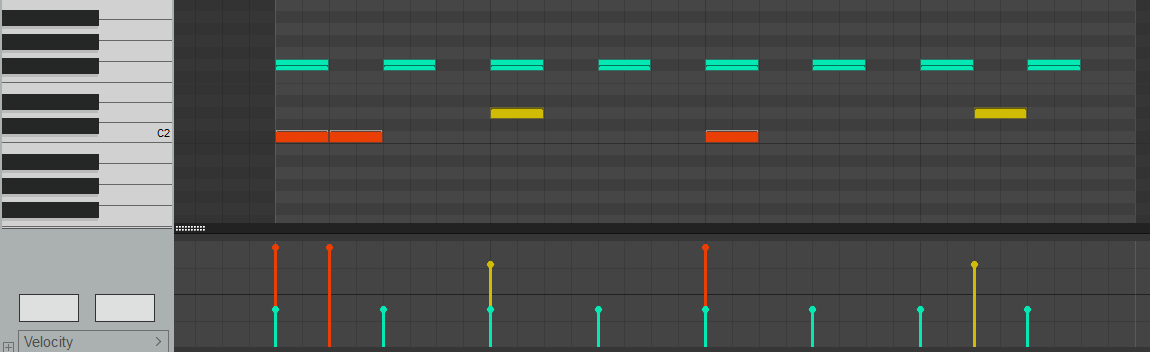
\includegraphics[width = 0.5\textwidth]{Imagenes/Bitmap/PatronPercusionBasico.png}
        \caption{Ejemplo de un patrón de percusión resultante.}
        \label{fig:PatronPercusionBasico}
    \end{figure}

    
    Una vez tenemos el ritmo base, podemos añadir algunos adornos. Algunos ejemplos de adornos podrían los \textit{drum fills} o las intros.

    \subsection{\textit{Drum Fills}}
    \label{subsubsec:generacion-drum-fills}

    Un \textit{drum fill} es un pequeño motivo musical que sirve para añadir variedad a un ritmo de batería y para hacer transiciones entre secciones de un arreglo musical\footnote{\url{https://es.wikipedia.org/wiki/Fill_(musica)}}. A veces los \textit{drum fills} pueden aparecer indicados en las partituras de los bateristas, pero en otras ocasiones sólo viene indicado dónde tocar un \textit{fill} y es el propio baterista el que improvisa un \textit{drum fill}.
    
    La primera idea para lograr tener \textit{drum fills} fue la de implementarlos como el resto de las partes de percusión. Esta idea fue descartada debido a que los \textit{drum fills} usan más elementos de la batería y son más creativos que los ritmos que hemos visto en el punto anterior.

    Por tanto, para obtener \textit{drum fills}, cargamos en REAPER (Sección \ref{sec:reaper}) un archivo MIDI (Sección \ref{subsec:que-es-midi}) con algunas notas de percusión marcadas. A continuación, añadimos a la pista el plugin arpegiador \textit{BlueArp} (Sección \ref{subsubsec:bluearp}) para que arpegie las notas de percusión del ítem MIDI cargado. Por último añadimos un plugin humanizador (Sección \ref{subsubsec:humanizador}) que además de variar la velocidad y \textit{timing} de las notas, varía la nota que se interpreta. Esto lo que hace en un instrumento de batería es cambiar que elemento de la batería se toca. Lo que obtenemos como resultado es una secuencia de golpes de batería generadas de forma aleatoria que al combinar con el ritmo base da como resultado un \textit{drum fill}.

    %TODO: referenciar esta imagen
    \begin{figure}[h]
        \centering
        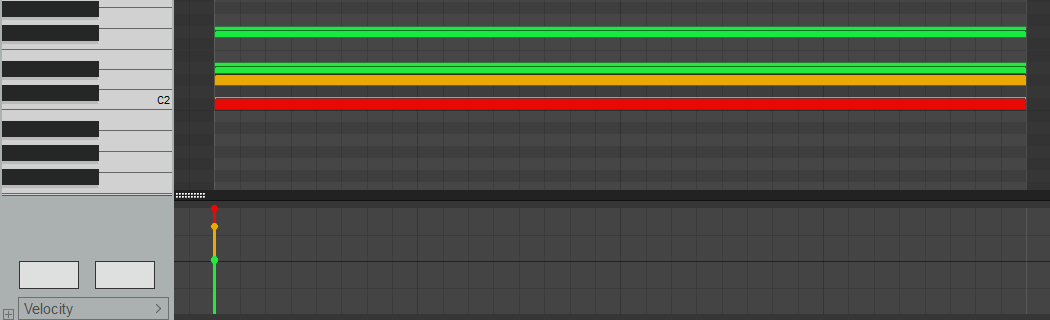
\includegraphics[width = 0.5\textwidth]{Imagenes/Bitmap/FillTemplate.png}
        \caption{Ítem MIDI auxiliar usado para generar \textit{drum fills}}
        \label{fig:FillTemplate}
    \end{figure}
    
    %TODO: referenciar esta imagen
    \begin{figure}[h]
        \centering
        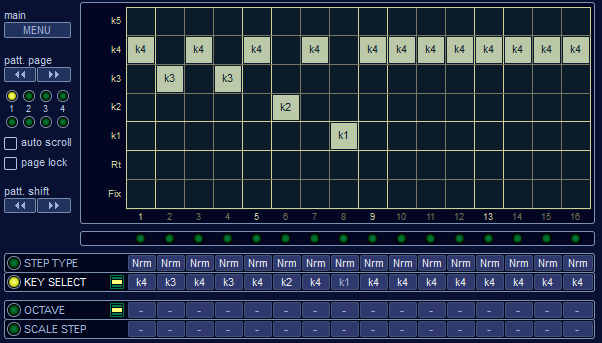
\includegraphics[width = 0.3\textwidth]{Imagenes/Bitmap/FillArp.png}
        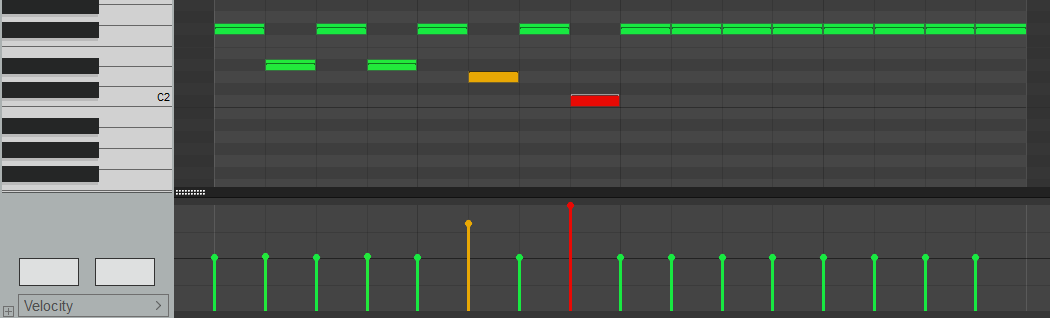
\includegraphics[width = 0.5\textwidth]{Imagenes/Bitmap/FillResult.png}
        \caption{Arpegiador y resultado final de un \textit{drum fill}}
        \label{fig:FillResult}
    \end{figure}

    Además, si esta secuencia que hemos generado suena sin el ritmo base, cumple la función de una intro de batería, que da pie a que entre el ritmo al comienzo del siguiente compás.

    Los \textit{drum fills} los colocaremos cada  4 compases, siendo cada 8 algo más largos, al igual que cuanto más avanzado se encuentren en la canción.


    
    
    \subsubsection{Estilos}
    \label{subsubsec:estilos-percusion}
    Todos los patrones que se generen serán variaciones de un patrón básico. Por ejemplo, en la Figura \ref{fig:Partituras-percusión} podemos ver un patrón básico de batería como el que vimos anteriormente y a su derecha un patrón de jazz. Si nos fijamos, podemos observar que el \textit{beat} y el \textit{engine} son similares, cambiando los golpes de percusión con los que se tocan dichas partes (platillos en ambos casos). 

    \begin{figure}[h]
        \centering
        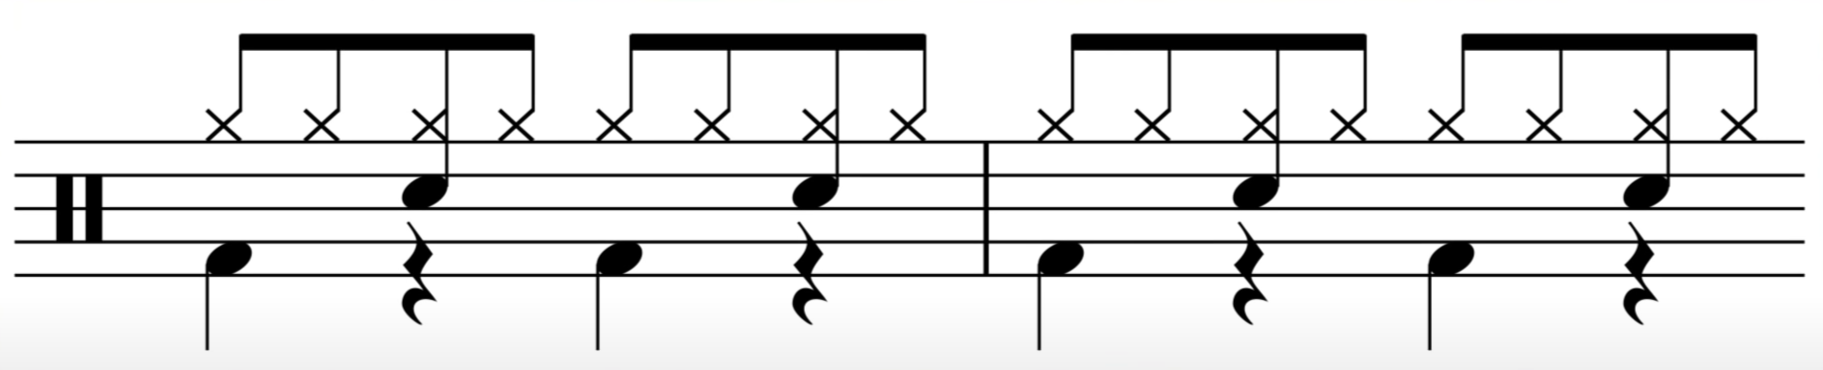
\includegraphics[width = 0.45\textwidth]{Imagenes/Bitmap/BateriaBasico.png}
        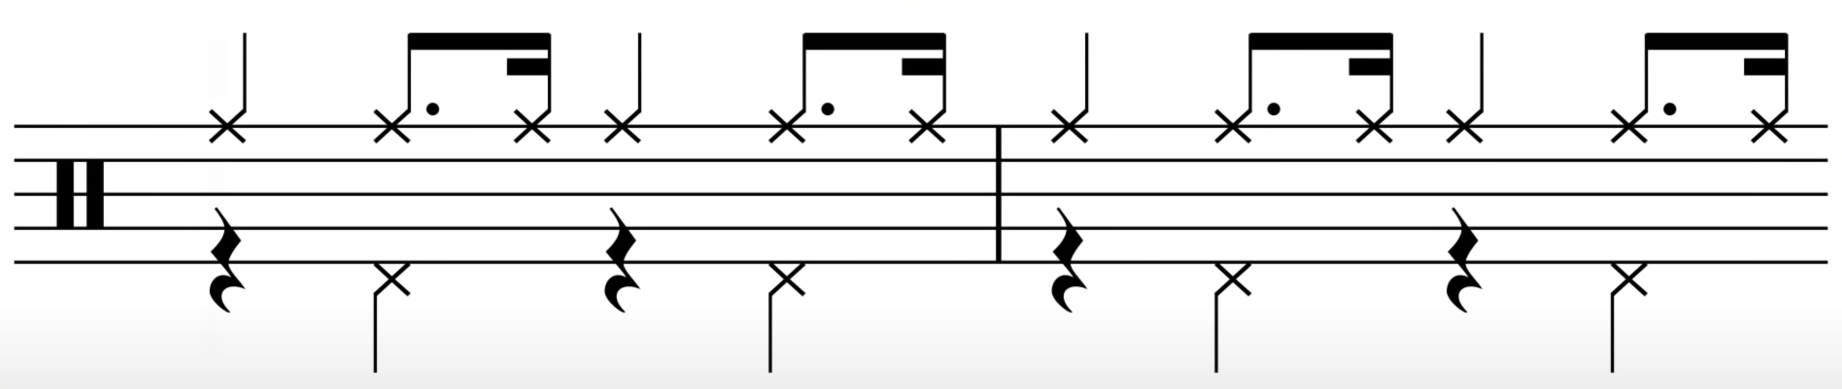
\includegraphics[width = 0.45\textwidth]{Imagenes/Bitmap/BateriaJazz.png}
        \caption{A la izquierda ritmo estándar básico de percusión, a la derecha ritmo estándar de jazz.}
        \label{fig:Partituras-percusión}
    \end{figure}
    
    Lo patrones básicos son los propios de varios géneros musicales. Con estos patrones tratamos de cubrir la mayor parte de ritmos posibles. Son los siguientes:
    
    \begin{itemize}
        \item \textbf{Estilo básico}: Ritmo más básico de bombo y caja con platillos como \textit{constant}.
        \item \textbf{Palmas}: Ritmo de palmas con varias voces simultaneas
        \item \textbf{Maracas}: Ritmo con una maraca como \textit{constant} con un bombo ocasional.
        \item \textbf{Jazz}: Platillos como \textit{beat} y haciendo un ritmo contrastante como \textit{constant} y un platillo de pedal haciendo el engine.
        \item \textbf{Disco}: Bombo a negras con caja y platillos.
        \item \textbf{Metal}: Platillos haciendo el \textit{beat} y doble bombo como \textit{constant}
        \item \textbf{Latin}: Bombo, caja y platillos haciendo ritmos que contrastan entre sí.
        \item \textbf{Rock}: Caja haciendo el \textit{beat} y bombo la \textit{constant}
        \item \textbf{Dembow}: Bombo y caja en el que cada segunda caja se retrasa ligeramente.
    \end{itemize}
    

    
    \subsubsection{Generación de patrones}
    \label{subsubsec:generacion-patrones}
    Para simplificar la representación interna a la hora de generar variedad entre patrones, generamos de forma independiente las partes del beat, del engine y del constant.
    
    Se parte de un patrón de batería básico, como los de la Figura \ref{fig:Partituras-percusión}. De manera aleatoria se decide saltarse algunas notas, adelantarlas, tocar dos veces en lugar de una, etc. De esta forma obtenemos un patrón de batería derivado de uno de los patrones básicos.

    Codificamos cada parte (\textit{beat}, \textit{engine} y \textit{constant}) como arrays de 16 unidades de tamaño y asignamos a cada elemento del array la duración de una semicorchea, por lo que el patrón resultante es un compás 4/4 dividido como máximo en semicorcheas. Variando ligeramente este patrón, crearemos otros dos que serán muy similares entre ellos y al original.

    \subsubsection{Combinación de patrones}
    \label{subsubsec:combinacion-patrones}
        
    Como se ha explicado en el punto anterior, hemos generado tres patrones distintos de un mismo estilo que además funcionan bien juntos. Llamaremos a estos patrones A, B y C.
    
    Es común en los arreglos de percusión combinar estos patrones de cierta manera para añadir variedad al ritmo básico. Por ejemplo, podemos encontrarnos una secuencia bastante común ABAC o una secuencia AABB, que no sería más que tocar de una en una en secuencia los patrones correspondientes, volviendo a empezar al llegar al final de la secuencia.
    
    Estas secuencias las generamos de manera aleatoria una vez, por lo que para cada canción generada saldrá una secuencia distinta pero a lo largo de una canción la batería mantiene esa secuencia continuamente.
    
    Dependiendo de la temática escogida para la canción, se cargarán unos estilos de batería u otros, generalmente tres estilos distintos que van cambiando a lo largo de la canción de manera aleatoria.

    
    %TODO: referenciar esta imagen
    \begin{figure}[h]
        \centering
        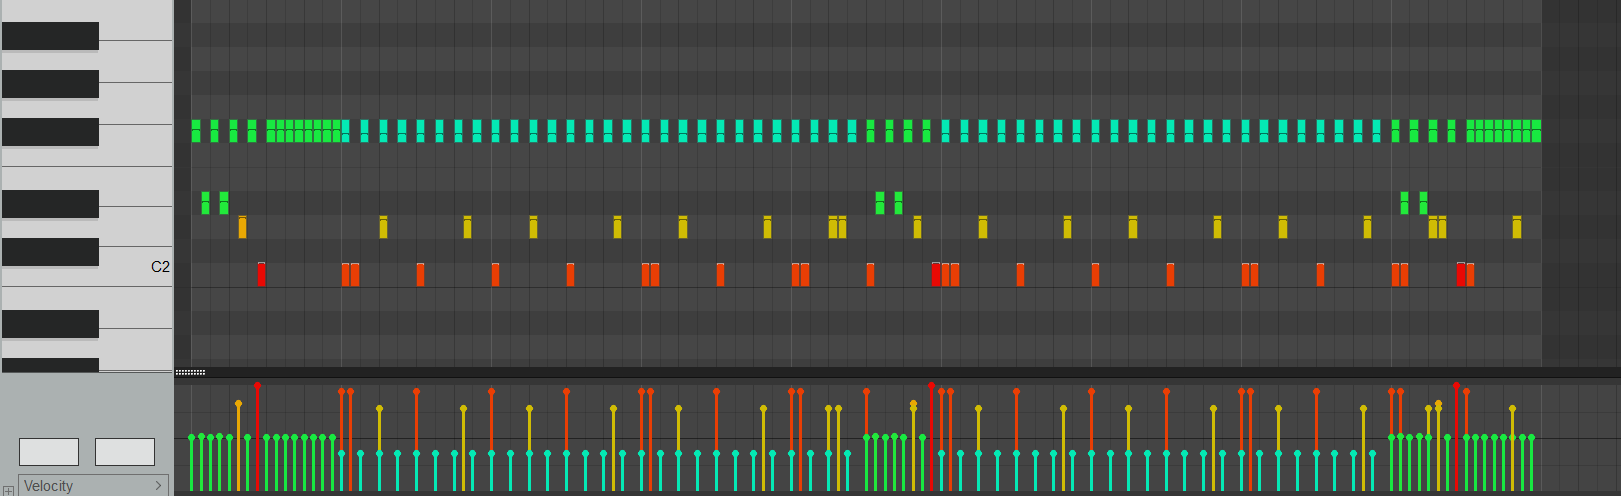
\includegraphics[width = 0.9\textwidth]{Imagenes/Bitmap/RitmoCompleto.png}
        \caption{Ritmo resultante completo}
        \label{fig:RitmoCompleto}
    \end{figure}
    
    \subsubsection{Percusión en MIDI}
    \label{subsubsec:percusion-midi}

A la hora de interpretar un archivo MIDI (Sección \ref{subsec:que-es-midi}) de percusión, la mayoría de instrumentos virtuales mapean las notas de la misma forma. Por ejemplo el bombo es la nota MIDI 36 y la caja la nota MIDI 38 (Do3 y Re3 respectivamente).

La velocidad de las notas MIDI en los instrumentos de percusión indican con cuanta fuerza se realiza el golpe. En algunos instrumentos virtuales la velocidad de la nota se ignora, en otros se reproduce el sonido correspondiente con más o menos volumen y en otros instrumentos hay muestras específicas grabadas para distintas velocidades de la nota. Asimismo, es común que en los instrumentos virtuales de percusión haya varias muestras para una misma nota y una misma velocidad, con el fin de que no suene siempre el mismo golpe exacto y el ritmo resultante suene más realista.
a\chapter{Sonorización del Proyecto}

\section{¿Qué es una DAW?}
\section{Instrumentos}

\subsection{¿Qué es un VST?}

\subsection{Presets}

\subsection{Instrumentos utilizados}

\section{REAPER}

\section{Temáticas musicales}

\section{Algoritmos de sonorización de MIDI}



\chapter{Cómo arreglar una canción}
Hacer un arreglo de una canción consiste en utilizar una idea musical, una composición o una canción entera para crear una canción nueva.

En nuestro caso vamos a usar un motivo o idea musical para arreglar una canción que funcione como música para un videojuego. Hay muchas formas de abordar esto, y como es común en la música y el arte, no hay una verdad absoluta.

Por nuestra parte, priorizamos que el arreglo funcione pero sea rico y variado, con varias secciones y sonidos posibles, de manera que dos generaciones distintas no sean nunca iguales. Bajo esta premisa, hemos definido una serie de normas para la estructura y timbres de la canción, que se generarán de manera pseudoaleatoria siguiendo dichas normas.

\section{Las partes fundamentales de una producción}
\label{sec:fundamentos-producccion-musical}

\section{Temáticas}
\label{sec:tematicas}

\section{Secciones}
\label{sec:secciones}

Dividimos la canción en un máximo de 8 secciones, las cuales tienen una duración de 8 compases cada una. Lo ideal para que una canción no se vuelva repetitiva es añadir o quitar elementos cada poco tiempo, siendo lo más común cada 8 compases.

El usuario puede, desde Reaper3, eligir si quiere renderizar la canción entera de 8 secciones, o seleccionar un rango se secciones para renderizar únicamente esas, ya que mientras sean secciones enteras y no se corten a la mitad, \textit{loopearan} de forma correcta sea cual sea la selección.

\section{Mezcla de melodías}
A la hora de elegir la melodía que sonará en cada sección, el usuario puede decidir si quiere mezclar la melodía o si usar siempre la versión original (\ref{cap:generacionMusical})
En el caso de que decida mezclar las melodías, generamos dos patrones adicionales de melodía combinando la melodía original trozeada, priorizando la repetición de uno de los trozos, seleccionado de forma aleatoria.

La repetición en la melodía es clave para que la canción sea predecible y sea fácil de recordar, objetivos que buscamos alcanzar usando patrones de repetición cortos, llegando a ser los patrones de un compás de duración los de menor longitud.

\section{Arpegios}
Arpegiar un acorde no es más que tocar las notas de dicho acorde de una en una en vez de todas a la vez, generalmente repitiendo un patrón sencillo que se repite constantemente. Por ejemplo, en un acorde de Do Mayor, si tocamos el acorde de la manera más simple tocaríamos las notas Do, Mi y Sol a la vez, mientras que si arpegiamos el acorde podríamos tocar con duración de una semicorchea la nota Mi, después Sol, luego Do y de nuevo Sol, y volveríamos a empezar la secuencia.

Para realizar estos arpegios a partir de los MIDIs de armonía (\ref{sec:arm:cuestion}) que ya tenemos, cargamos un plugin  \textit{BlueArp} (\ref{subsubsec:bluearp}) con varios arpegios diseñados por nosotros, de los cuales se seleccionará uno de manera aleatoria.

\section{Línea de bajo}\label{sec:lineas-de-bajo}
Al comienzo del desarrollo de la herramienta, implementamos un generador de líneas de bajo que crea, a partir de una armonía referencia dada, una melodía monofónica para ser interpretado por el bajo, usando principalmente la nota más grave de cada acorde (que puede no ser la fundamental, ya que la armonía puede tener inversiones de acordes). Este generador es similar al generador de baterías (\ref{subsec:generacion-percusion-propia}) pero simplificado.

Este algoritmo tenía algunas limitaciones y a la hora de ampliarlo para añadir variedad, descubrimos una alternativa más cómoda y flexible.

En la versión actual de la herramienta, cargamos la armonía (\ref{sec:arm:cuestion} (sin inversiones) en Reaper en la pista de bajo y utilizamos el plugin \textit{BlueArp} (\ref{subsubsec:bluearp}) para interpretar la línea de bajo usando principalmente la nota fundamental del acorde y en ocasiones el resto de notas de dicho acorde.

\section{Arreglos de batería}
Dependiendo del estilo de la canción (\ref{sec:tematica}), se genera cada cuatro compases de forma aleatoria un estilo de batería o género musical de entre hasta tres posibles. Se cargan alternando las 3 variaciones distintas que nos proporciona el generador de baterías (\ref{subsec:generacion-percusion-propia}) formando un patrón calculado de forma aleatoria una única vez. Por ejemplo si el patrón calculado es ABAC, patrón típico de batería, cargaríamos el MIDI correspondiente al ritmo A, de longitud de un compás, a continuación el ritmo B, de nuevo el A y después el C. Y repetiríamos el mismo patrón ABAC durante toda la canción.

\section{\textit{Ear candy}}
\label{sec:ear-candy}
El \textit{ear candy} en la producción musical son pequeños elementos que se añaden a una canción para volverla más interesante, que no son imprescindibles para la canción, pero que captan la atención del oyente o ayudan a dar coherencia a la mezcla. Podríamos decir que el \textit{ear candy} es la guinda del pastel en una canción.

A partir del arreglo inicial, nuestro programa sigue unas reglas para añadir varios tipos de \textit{ear candy}: transiciones, \textit{drum fills} y sonidos adicionales que enriquecen la mezcla final:


\begin{itemize}

\item Transiciones: cuando una sección contiene un número determinado de instrumentos sonando simultáneamente y la sección siguiente contiene al menos un instrumento más, se añade un \textit{riser} formado a partir de un sonido aleatorio con mucha reverb que va aumentando en volumen según nos acercamos al cambio de sección. En el caso contrario, es decir, que haya varios elementos en una sección y en la siguiente al menos 2 elementos menos, se agrega un \textit{downriser}, que no es más que un sonido reverberado también pero esta vez decreciente en volumen.

\item \textit{Drum fill}: (\ref{subsubsec:drum-fills}) Cuando va a entrar un instrumento de batería en la próxima sección, y sólo si no hay un \textit{riser} colocado para la transición, se coloca un \textit{drum fill} que sonando sin otros instrumentos de batería, funciona como un ritmo de introducción al patrón de batería. Adicionalmente, cada 4 compases de percusión, colocamos un \textit{drum fill} que suena a la vez que el ritmo principal para añadirle movimiento, siendo de mayor duración en los compases múltiplos de 8 y cuanto más avanzados en la canción estemos.

\item  Entrada adelantada de sonidos: Si entre dos secciones no hay ningún elemento común, uno de los elementos adelanta su entrada para que el cambio no sea muy brusco. Al elegir instrumento para hacer esto, tiene prioridad el instrumento de bajo. Si no hay bajo presente, será la melodía o el acompañamiento el que resuelva esto, en ese orden de prioridad.

\item  Sonidos adicionales: Si en una sección no hay muchos sonidos presentes, se agregarán de forma aleatorio algunos sonidos (con más o menos protagonismo en la mezcla) a lo largo de la sección.


\end{itemize}

\section{Arreglo}
\label{sec:arreglo}

Generamos una matriz de booleanos de 7x8 la cuál rellenamos de maneras aleatoria, y que posteriormente corregimos siguiendo unas normas:

\begin{itemize}

\item No puede haber dos pistas de acompañamiento sonando simultáneamente.
\item En la primera sección no puede haber más de tres instrumentos principales (\ref{subsec:instrumentos-secundarios}) sonando a la vez.
\end{itemize}

\section{Pistas}\label{sec:pistas}

Dependiendo de la temática (\ref{sec:tematicas}) de la canción, la herramienta cargará en Reaper varios efectos (\ref{subsec:plugin}) por pista, la mayoría son genéricos dependiendo de la temática y pista concreta, pero el instrumento que interpretará el MIDI(\ref{subsec:que-es-midi}) cargado se seleccionará de manera aleatoria de entre unos plugins vst (\ref{subsec:plugins-utilizados}) seleccionados por nosotros.

\subsection{Instrumentos principales}
\label{subsec:instrumentos-principales}
Estos instrumentos son los que harán sonar la matriz del arreglo(\ref{sec:arreglo}). Cubren las necesidades básicas de toda producción (\ref{sec:fundamentos-producccion-musical}) y son los siguientes:

\begin{itemize}
\item 2 pistas de melodía, una de ellas una octava por encima de la otra. En esta pista van los MIDIs de melodía (\ref{sec:como-generamos-melodias})
\item 2 pistas de acompañamiento. No pueden sonar al mismo tiempo (ver arreglo(\ref{sec:arreglo})). Estas pistas van acompañadas de un arpegiador \textit{BlueArp}(\ref{subsubsec:bluearp}) que hará que en ocasiones los acordes sean arpegiados o tocados con otro ritmo distinto al del MIDI. Estas pistas cargan el MIDI de armonía (\ref{sec:arm:cuestion})
\item Una pista de pads. Esta pista carga el MIDI de armonía (\ref{sec:arm:cuestion}), por lo que interpreta los acordes de la canción. Cuando suena sin el acompañamiento hace la propia función de acompañar a la melodía algo más en segundo plano, y cuando suena a la vez que el acompañamiento complementa el sonido de este.
\item Una pista de bajo. Esta pista carga el MIDI de armonía (\ref{sec:arm:cuestion}) pero esta vez sin inversiones (\ref{sec:arm:acordes})). Esto es porque en el bajo generalmente queremos una melodía monofónica con las notas fundamentales de cada acorde, y necesitamos que la fundamental sea la nota más grave porque le metemos un arpegiador \textit{BlueArp}(\ref{subsubsec:bluearp}) para tocar o bien únicamente esa nota, o un arpegio o una línea de bajo.
\item Una pista de batería. Esta pista carga varios MIDIs de batería (\ref{subsec:generacion-percusion-propia}) dependiendo de la temática de la canción (\ref{sec:tematica})
\end{itemize}

\subsection{Instrumentos secundarios}
\label{subsec:instrumentos-secundarios}
Estos instrumentos son los que generarán los sonidos de los \textit{ear candy} (\ref{sec:ear-candy}) a partir de la disposición del arreglo, sin ser los propios sonidos de este. Son sonidos que no acaparan el protagonismo, más bien se encuentran en un segundo plano y es fácil que no te des cuenta de que están ahí, pero hacen una diferencia significativa a la hora de dar cohesión y dinamismo a una canción. Son los siguientes:


\begin{itemize}
\item 2 pistas de \textit{uprisers}. Cargan el MIDI de acompañamiento para crear transiciones usando un sonido reverberado que deja de sonar al entrar la nueva sección. Sólo puede sonar una simultáneamente, son dos para añadir variedad.

\item 2 pistas de \textit{downrisers}. Al igual que los uprisers, cargan el MIDI de acompañamiento pero esta vez para generar una bajada, usando una Reverb con menos ataque (alcanza más volumen antes) que baja de volumen progresivamente.

\item Una pista de \textit{drum fills} (\ref{subsubsec:drum-fills}). Suenan de forma simultánea a las baterías o cuando va a entrar una sección con batería y no estaba sonando en la sección actual. Carga un MIDI especial que tiene marcadas las notas de bombo, caja y dos platillos, que serán interpretados por el arpegiador \textit{BlueArp}(\ref{subsubsec:bluearp}) y con el humanizador(\ref{subsubsec:humanizador}) configurado con algo de aleatoriedad en el pitch, lo que en instrumentos de batería significa que sonarán distintos golpes (cajas, platillos, toms, palmas) cada vez.

\item 4 pistas de sonidos puntuales (\ref{sec:ear-candy}). Cargan el MIDI de la armonía y suenan al menos dos veces por sección (\ref{sec:secciones}) durante un periodo corto de tiempo si la sección cumple los requisitos planteado en la sección de \textit{ear candy}. Usan un arpegiador \textit{BlueArp}(\ref{subsubsec:bluearp}) para interpretar una melodía tocando las notas presentes en el acorde y llevan un efecto de delay creado con el plugin \textit{CRMBL} \ref{subsubsec:delay}.
\end{itemize}


\chapter{Interfaz de Usuario con TKInter}
\label{cap:GUIconTKInter}
Hemos elegido TKINter como frontend para nuestra aplicación. El frontend es la parte visible de una aplicación, con la que puede interactuar el usuario.

\section{TKInter}
\label{sec:TK}
\href{https://docs.python.org/es/3/library/tkinter.html}{TKInter} es la biblioteca por defecto que trae Python para la creación de GUI, interfaaz gráfica de usuario por sus siglas en inglés.

Al venir integrado con python, es una herramienta de fácil inclusión en los proyectos que usen python. TKInter brinda una interfaz fácil de usar, pero muy sencilla en cuanto a posibilidades. Hemos priorizado la funcionalidad frente a la estética, política que casa muy bien con TKInter.

\subsection{Widgets de TKInter}
Los \textit{widgets} de TKInter son elementos de UI a los que se les puede vincular acciones de código propio. Estos \textit{widgets} van asociados a una ventana para poder renderizarse en pantalla y así recibir acciones del usuario o mostrar información. Veremos en las subsecciones siguientes las funciones de la aplicación, los widgets asociados y el funcionamiento de nuestra aplicación por debajo.

\subsection{Sistema de pestañas con Tk.Notebook}
\textit{Tk.Notebook} es un \textit{widget} que permite tener varias pestañas en la aplicación. Esto se hace creando una nueva ventana y pasándosela al \textit{Notebook} para que las organice. Esto nos deja la posibilidad de organizar y distribuir las funcionalidades de la aplicación en distintas pestañas como son: \generationTabName{}, \tematicTabName{}, \advancedTabName{}, \configTabName{}.

% Se puede cambiar el título del capítulo por La App y dejar la GUI como sección
\section{La app}
\label{sec:TK:app}

\subsection{Generación Musical}
Pestaña de la aplicación que permite generar el MIDI. Esto se realiza vinculando los \textit{widgets} de botón de TKInter con los apartados de generación y armonía.

** referencias a generación de Rodrigo y armonización de VM **

\subsection{Temáticas y sonorización}
\label{subsec:TK:TematicasYSonorizacion}
La pestaña \tematicTabName{} anexiona las principales funcionalidades de la aplicación. El MIDI generado en la pestaña \generationTabName{} se sonoriza de acuerdo a la configuración de la pestaña \tematicTabName{}. 

**referencias a Sonorización de Javi**

\subsubsection{Semilla}
La semilla es la fuente de generador aleatoria que permite obtener los mismos valores cuando se obtiene un nuevo \textit{random()} de un generador.

Nos interesa poder generar distintas semillas, que den variedad a los resultados generados por la aplicación. Conociendo que semilla se ha generado, podemos guardarlas (ver \nameref{subsub:TK:serializacionYPresets}).

** referncia a arreglos en REAPER de Javi **

\subsubsection{Serialización y presets}
\label{subsub:TK:serializacionYPresets}
La aplicación cuenta con la posibilidad de guardar su estado en momentos específicos. Esto lo hacemos leyendo los atributos de una clase llamada AppModeState y serializándolos a un objeto Json. Una vez tenemos este objeto Json, lo persistimos a un fichero .json con un nombre que nos de el usuario. Estos ficheros que guardan la configuración del estado de la aplicación reciben el nombre de \textit{presets}. 

Estos presets pueden ser recuperados para establecer el estado de la aplicación a la información contenida en el json. Esta característica permite al usuario guardar la configuración de temática, checkboxes (modificadores) y semillas que quiera recuperar possteriormente.

\subsection{Modo avanzado}
La pestaña \advancedTabName{} de la aplicación dota al usuario de un control más exhaustivo de la aplicación. Esta pestaña está apartada del público general debido a que ofrece una visión más compleja de la aplicación, estando dirigida a usuarios de la aplicación avanzados o personas con conocimientos musicales avanzados.

\subsection{Configuración y guardado}
Debido a que dependemos de software de terceros como es REAPER y no podemos brindarlo con nuestra aplicación, necesitamos que el usuario nos brinde información acerca de su sistema, como en qué ruta se encuentra el ejecutable de REAPER para poder iniciarlo y hacer uso de nuestra aplicación

\chapter{Manual de Usuario}
\label{cap:descripcionTrabajo}

En este capítulo recogeremos los pasos que debe seguir un usuario para poder utilizar la aplicación. Además de las \refname{sec:dependeciasApp}, se explican los dos grandes pasos que hay que tomar para generar un tema con nuestra aplicación. 

Estos dos grandes pasos son la \nameref{sec:dependeciasApp} y la \nameref{sec:instrumentalizacion} del contenido generado en el primer paso. 

\section{Dependencias de la aplicación}
\label{sec:dependeciasApp}
\subsection{Dependencias de Instalación}
	Para ver todas las dependencias, consultar el Apéndice \ref{Appendix:Key1}

	Para hacer uso de la aplicación, se requiere instalar herramientas de terceros que permiten el uso de nuestro asistente de composición musical.
	Estas dependencias se componen desde lenguajes de programación tales como Python y JavaScript hasta los instrumentos que permiten poder escuchar los temas musicales generados.

\subsection{Interfaz gráfica con TKInter}
	TKInter es la interfaz por defecto que \PythonLink{} ofrece a los desarrolladores para montar una GUI (Interfaz Gráfica de Usuario por sus siglas en ingles).
	Esta herramienta viene integrada junto con Python, por lo que no requiere instalar ningún entorno ni herramienta adicional para hacer uso de ella.



\subsection{REAPER}
\label{subsec:reaper}
	\href{https://www.reaper.fm/}{REAPER} es el DAW de producción musical que usamos en nuestra aplicación
	Un DAW, \textit{Digital Audio Workstation}, es una estación trabajo de audio digital.

	Este entorno de edición y producción musical es el que nos permite sonorizar el audio que generamos en nuestra aplicación. Es decir, nos permite agregar los instrumentos y efectos de audio que hacen sonar el MIDI almacenado. 

\section{Generación de audio}
\label{sec:generacionAudio}
	Generación de audio
\section{Instrumentalizacion}
\label{sec:instrumentalizacion}
	Instrumentalizacion
	
%\include{Capitulos/Capitulo5}
\chapter{Conclusiones y Trabajo Futuro}
\label{cap:conclusiones}

Conclusiones del trabajo y líneas de trabajo futuro.

Antes de la entrega de actas de cada convocatoria, en el plazo que se indica en el calendario de los trabajos de fin de grado, el estudiante entregará en el Campus Virtual la versión final de la memoria en PDF.




%%%%%%%%%%%%%%%%%%%%%%%%%%%%%%%%%%%%%%%%%%%%%%%%%%%%%%%%%%%%%%%%%%%%%%%%%%%
% Si el TFG se escribe en inglés, comentar las siguientes líneas 
% porque no es necesario incluir nuevamente las Conclusiones en inglés
\begin{otherlanguage}{english}
\chapter*{Introduction}
\label{cap:introduction}
\addcontentsline{toc}{chapter}{Introduction}

Introduction to the subject area. This chapter contains the translation of Chapter \ref{cap:introduccion}.

\section{Motivación}
Our main purpose for this project is to make music composition, focused primarily on video games, to users with low or non existent musical knowledge.

In order to reach this purpose, we want to rely on the field of Artificial Intelligence, exploring techniques and methodologies to be able to generate something that is interesting.

\section{Objectives}
With our purpose defined, the next steps is to define a series of objectives:
\begin{enumerate}
    \item Generate melodies through the use of different tools, including \textit{Machine Learning} or stochastic algorithms.
    \item Harmonize the melody previously generated in a way that results pleasant to the human ear, either through the use of Artificial Intelligence or own heuristics.
    \item Sound the generated music notes making a property selection of instruments, choosing between pre-defined themes. 
    \item Create an application for \textit{Windows} that allows the user to apply this techniques in a friendly way.
\end{enumerate}

\section{Plan de trabajo}
El tener objetivos claramente separados en cuanto a funcionalidad, nos permite separar el trabajo de manera más eficiente en módulos independientes, como una cadena de producción separada en etapas que se une en la app final. 

\begin{enumerate}
    \item Investigación y estudio del campo de la Inteligencia Artificial aplicada a la generación musical. Durante esta fase, revisaremos la literatura existente, investigaremos los enfoques y algoritmos más relevantes y nos familiarizaremos con las herramientas y recursos disponibles.
    \item Desarrollo del algoritmo de generación de melodías. Utilizaremos técnicas de aprendizaje automático y modelado generativo para crear un sistema capaz de componer melodías originales y variadas.
    \item Implementación de la armonización de las melodías generadas. En esta etapa, diseñaremos y desarrollaremos heurísticas y reglas musicales para armonizar las melodías de manera coherente y agradable al oído.
    \item Selección y configuración de instrumentos. Investigaremos y seleccionaremos una variedad de instrumentos musicales virtuales que se ajusten a las temáticas predefinidas de los videojuegos. Configuraremos estos instrumentos para que reproduzcan las melodías generadas de manera convincente al oído humano.
    \item Desarrollo de la aplicación de escritorio. Utilizaremos las tecnologías adecuadas para desarrollar una interfaz de usuario intuitiva y amigable que permita a los usuarios generar, armonizar y sonorizar sus propias composiciones musicales para videojuegos.
\end{enumerate}








\chapter*{Conclusions and Future Work}
\label{cap:conclusions}
\addcontentsline{toc}{chapter}{Conclusions and Future Work}

Conclusions and future lines of work. This chapter contains the translation of Chapter \ref{cap:conclusiones}.



\end{otherlanguage}
%%%%%%%%%%%%%%%%%%%%%%%%%%%%%%%%%%%%%%%%%%%%%%%%%%%%%%%%%%%%%%%%%%%%%%%%%%%

\chapter*{Contribuciones Personales}
\label{cap:contribucionesPersonales}
\addcontentsline{toc}{chapter}{Contribuciones Personales}

\section*{Rodrigo Sánchez Torres}
\subsection*{Procesamiento de datos}
Para poder utilizar algoritmos de inteligencia artificial en nuestro trabajo era necesario tener un dataset limpio y adecuado para nuestros objetivos.

La primera tarea fue buscar un dataset que contenga información sobre melodías. En la búsqueda se valoraron muchos tipos de datasets, finalmente, en la exploración de los datasets de Magenta se decidió utilizar el \textit{Bach Doodle Dataset}.

Una vez elegido el dataset se procedió al tratamiento de este, con distintos acercamientos se fueron realizando limpiezas en principio superficiales, pero pronto se decidió que lo mejor era tener un dataset con solamente melodías que estén en la misma escala e incluso en un rango reducido de octavas. 

También se exploraron las opciones de usar o no silencios, siendo en algoritmos como cadenas de Markov mejor no emplear silencios, pero en redes neuronales recurrentes se obtuvieron mejores resultados con silencios en el dataset.

Finalmente se testeó tanto a usar tiempos absolutos en segundos como a normalizar el tiempo utilizando \textit{steps} y BPM (\textit{beats per minute}), dando mejor resultado tener el tiempo normalizado y homogéneo en el dataset.

\subsection*{Algoritmos de \textit{Machine Learning}}
Antes de poder elegir qué modelos serían más adecuados para la generación de melodías fue necesario realizar una amplia investigación sobre el tema, para poder conocer la mayor cantidad de técnicas y modelos que podemos aplicar a nuestro trabajo.

Tras la investigación quedó claro que era necesario buscar un modelo que no fuera determinista, para poder generar melodías diferentes en cada ejecución. Es por esto que se decidió explorar los 3 modelos actuales: cadenas de Markov, redes neuronales recurrentes con capa \textit{softmax} y modelos de Magenta.

En primer lugar se empezó a explorar la generación con Markov, para esto se realizó una investigación sobre el tema y sus posibles aplicaciones. Para poder utilizar correctamente las cadenas se utilizó una notación común a lo largo del proyecto en los algoritmos propios de generación, como era \textit{"pitch\_duration"}.

Para poder utilizar cadenas de Markov se procesó manualmente el dataset, creando matrices de transición que sean interpretables por la librería utilizada. Finalmente, se consiguió tener un primer modelo de generación listo, que permitió continuar el desarrollo de otras ramas que se apoyan en éste.

Una vez se tuvo el primer modelo de generación listo se podía dedicar más tiempo a desarrollar un modelo más complejo. Se decidió utilizar entonces una red neuronal recurrente. Pero esta tenía el problema de ser un modelo determinista, así que se añadió finalmente una capa \textit{softmax}, que permitía introducir una aleatoriedad a la generación controlada con un parámetro de temperatura.

Este modelo fue el más complejo de desarrollar, pues había que realizar mucho trabajo de ajuste de \textit{súperparámetros} y diseño de la propia red. Además, se realizaron varias modificaciones al dataset, que finalmente no aportaban un mejor resultado. Al final tras un largo período de prueba ser decidió adoptar el diseño actual, teniendo una entrada de número reales, con el \textit{pitch}, duración y tiempo de inicio de la nota actual, y una salida con valores de tipo \textit{label}, siendo estas las posibles notas que podía elegir la red. Al utilizar salida con valores de tipo \textit{label} codificados mediantes \textit{one-hot encoding} se podía utilizar la capa \textit{softmax} mencionada anteriormente.

La red conseguía finalmente un rendimiento aceptable, por lo que se realizaron pruebas para entrenarla de forma que indicara también el tiempo de inicio de cada nota, lo que podía generar melodías más interesantes sobre el papel. Sin embargo, la red no conseguía aprender patrones significativos sobre este, obteniendo una precisión tan baja que no merecía la pena utilizar dicho parámetro. Es por esto que se decidió introducir los silencios como notas adicionales. 

Este modelo consiguió una generación mucho mejor a las cadenas de Markov, manteniendo patrones más típicos en la composición pero con limitaciones. Aún así se decidió mantener el modelo con Markov para tener una generación más experimental.

Intercalado con el desarrollo de la red neuronal recurrente se integró Magenta al proyecto, con el fin de proporcionar una generación más elaborada que la de Markov para poder trabajar en otras ramas y producir mejores resultados. 

La integración de Magenta supuso una gran cantidad de problemas, pues principalmente no se podía utilizar el paquete de Python en Windows. Tras realizar varias pruebas con binarios precompilados para Windows, migraciones a Ubuntu y diversos acercamientos se decidió que no era viable utilizar el paquete de Python, por lo que se exploró el uso del paquete de JavaScript.

El principal conflicto era que el proyecto estaba íntegramente desarrollado en Python, por lo que el módulo de JavaScript tenía que estar separado de éste. Finalmente se consiguió comunicar el proyecto con un script (magentaPython.py) que actúa de puente entre Python y JavaScript. Este script utiliza el módulo \textit{subproccess} para lanzar un proceso de JavaScript, con el que nos podemos comunicar por medio de argumentos de dicho proceso y la salida estándar de éste. Con esta metodología podemos mandar melodías serializadas en JSON al proceso y recibir resultados de generación recogiendo la salida estándar con el mismo formato JSON.

Este acercamiento permite utilizar Magenta en la aplicación, pero conlleva otros problemas de dependencia de paquetes y sobre todo de una conexión a internet para utilizar los modelos alojados en la base de datos de Google.

\subsection*{Aportaciones a la aplicación}
Además, se han realizado aportaciones al código de la aplicación. Se han introducido los módulos de generación a ésta, así como la posibilidad de elegir uno u otro desde código. También se han añadido las funcionalidades de carga de melodías existentes y guardado de una melodía generada, pudiendo elegir el nombre y ubicación del archivo.

\section*{Víctor Manuel Estremera Herranz}

Antes de empezar con las técnicas de armonización utilizadas, falta un paso previo crucial. Y es la creación de una estructura de clases y métodos que den soporte a todo lo explicado en el apartado \ref{sec:arm:armonia}. Existen clases que abstraen lo que representa una nota musical (\ref{arm:notas_musicales}), un intervalo (\ref{sec:arm:intervalos}), una escala (\ref{sec:arm:escalas}) y la armonía de una escala (\ref{arm:armonia_escala}) tal como se ha explicado. Un acorde (\ref{sec:arm:acordes}) es respresentado también como una escala. 

Al menos dos páginas con las contribuciones del estudiante 2. En caso de que haya más estudiantes, copia y pega una de estas secciones.

\section*{Javier Callejo Herrero}
\subsection*{Generación de percusiones.}
Lo primero que se hizo fue investigar los diferentes modelos de Magenta, tanto para tomar ideas como para decidir si podíamos usar dichos modelos en nuestra herramienta. 

Una vez vistas las herramientas disponibles, se decidió que los resultados obtenidos no ofrecían la variedad que requería la herramienta, por lo que se implementó un generador de percusión propio. Este generador permite crear patrones de batería de varios géneros distintos (como el jazz, el rock, la música disco, etc.) Estos patrones generados nos servirán para las siguientes partes del trabajo, en concreto la del diseño de temáticas.

\subsection*{Generación de líneas de bajo.}
Tras haber implementado el generador de percusión, se implementó una primera versión de un generador de líneas de bajo, que cogía un ítem MIDI con acordes y usaba las notas más graves para crear de forma pseudoaleatoria una melodía monofónica que si  sirviera como línea de bajo. Más adelante se descartó el uso de este generador al descubrir formas mejores de afrontar este programa (el uso de un plugin arpegiador).

\subsection*{Selección de plugins.}
De forma paralela a los apartados anteriores, se realiza una investigación exhaustiva de plugins (de instrumentos virtuales principalmente). Continuamente nos encontramos con problemas de almacenamiento e instalación muy tediosa.

Es más adelante cuando se reúnen finalmente todos los plugins de instrumentos virtuales que se usarán en la herramienta, plugins ligeros, de fácil instalación, pues son colocados los .vst o .dll en una única carpeta comprimida para facilitar la instalación tanto al usuario final como a los propios compañeros del trabajo.

\subsection*{Programar en Reaper.}
Se investiga el uso de ReaScript con Python para comenzar a automatizar tareas en Reaper. Primeramente se logran cargar instrumentos virtuales e ítems MIDI llamando a un script desde una acción de Reaper.

A continuación, se diseña y se implementa la carga de plugins que cubren las necesidades concretas de cada pista. (Se continúa buscando plugins que cubran nuestras necesidades, en particular plugins de efectos).

Desde ahí, se comienza a desarrollar una arquitectura que permite crear un arreglo para la primera temática (pradera). En este punto tenemos un script que carga ítems MIDI de melodía, armonía, batería y bajo. Además, añade de forma pseudoaleatoria plugins a las pistas y al máster: tenemos las primeras canciones generadas.

En este momento se empiezan a diseñar las temáticas. Se habla de ello en el siguiente apartado.

Se continúa hasta tener todas las temáticas programadas, añadiendo progresivamente mejoras y funcionalidades nuevas, como el subir o bajar semitonos, añadir diversos efectos a la mezcla o, finalmente, cambiar la complejidad de la melodía cargada.

Cabe destacar que existe una investigación sobre conectar scripts externos con Reaper, pero no se logra dicho objetivo y pasa a un segundo plano hasta más avanzado el desarrollo (Sección de Miguel Comunicación entre Vanguard Music y Reaper).

\subsection*{Diseño e implementación de las temáticas.}
Se investigan los elementos tanto técnicos como creativos necesarios para crear las distintas temáticas para las canciones. A continuación, se diseñan e implementan en Reaper todas las temáticas que están disponibles en la herramienta.

Para la implementación de las temáticas, ha sido requerido un exhaustivo trabajo de selección de timbres usando los instrumentos virtuales disponibles. El proceso es el siguiente: selección de plugin, elección o diseño del timbre dentro del plugin, guardado de un preset de Reaper y adición de dicho preset al script de Python para su posterior recuperación al lanzar el script en Reaper.

\subsection*{Diseño de la interfaz gráfica.}
Finalmente, se renderizaron en 3D usando Blender los diversos fondos presentes en la pestaña de sonorización de la aplicación y se colocaron en TKInter.


\section*{Miguel González Pérez}

\subsection*{Primera aproximación a la generación de MIDI con Magenta.}
Uno de los primeros objetivos era conseguir generar melodías con música simbólica a través de la herramienta de Magenta. Dado que no fue posible para nosotros utilizar la API de Magenta desde Python en Windows, surgió la alternativa de utilizar la API de JavaScript, lo que implicaba integrar Node.js con el resto del desarrollo en Python. 

Si bien logramos adquirir la melodía en forma de NoteSequence de Magenta en el contexto de JavaScript, no podíamos acceder a ello desde Python, por lo que más tarde se encargaría mi compañero Rodrigo de continuar y completar esta tarea.

\subsection*{Arquitectura de la Aplicación en TKInter.}
Tras el anterior apartado, mi siguiente tarea fue la de montar la arquitectura de la aplicación en TKInter con Python. Gran parte del trabajo en este apartado fue el del estudio de la documentación de \textit{TKInter}, la biblioteca estándar de Python para la creación de interfaces gráficas. 

Utilizando estos conocimientos, diseñé la aplicación de forma que disgregase las funcionalidades principales en pestañas diferenciadas. Esto requería en cuanto a implementación diseñar el código de forma que gestionar y añadir varias pestañas fuera escalable y sostenible.

El mantenimiento de un estado interno de la aplicación durante la ejecución y la posterior serialización a JSON y persistencia en ficheros en forma de presets son parte del trabajo que he realizado en el desarrollo de la aplicación. De este estado interno se sustrae la información necesaria, como temáticas y semillas, para la instrumentalización en Reaper. Esto implica también recuperar las configuraciones del estado interno de la aplicación guardadas por el usuario, de forma que no produzca errores.

La configuración propia de la aplicación, como la ruta al ejecutable de Reaper, también fue parte de este proceso de persistencia en formato JSON.

Para el desarrollo de la aplicación he aplicado algunos patrones de diseño software, como \textit{Strategy} a la hora de asignar el generador musical en la pestaña \textit{avanzado} o el propio sistema de pestañas de la aplicación, que aplica el patrón \textit{State} para manejar la entrado, actualización y salida de cada módulo de la aplicación.

En un momento avanzado del desarrollo de la aplicación, encontramos la necesidad de explicar los distintos elementos de la interfaz de usuario de la aplicación de forma rápida y sencilla. Para esto se creó la clase \textit{Tooltip} que permitía mostrar un pequeño texto cuando pasabas el ratón por encima de un elemento de la interfaz. Más tarde, cuando la aplicación evolucionó, optamos por usar un plugin de TKInter que traía \textit{tooltips} integradas que funcionaban mejor, adaptándose al tema oscuro de la aplicación.

\subsection*{Comunicación entre Vanguard Music y Reaper.}
Uno de los principales retos de la aplicación era la comunicación con Reaper. Nuestra intención inicial era la de permitir al usuario utilizar la aplicación sin tener que preocuparse en exceso por Reaper. Esto planteaba varios desafíos, siendo uno de ellos el de añadir nuestros scripts de ejecución sin necesidad de que el usuario tenga que registrarlos manualmente en Reaper. 

Reaper permite la ejecución de scripts en Python, \textit{LUA} y \textit{EEL} a través de su API \textit{ReaScript}. No obstante, estos scripts tienen que haber sido registrados en Reaper antes de poder ser ejecutad. Si bien éramos capaces de ejecutar los scripts ya registrados en Reaper desde nuestra aplicación gracias al trabajo de Javi, no podíamos registrar nuevos scripts desde código. Mi trabajo en esta sección fue la de estudiar la documentación de \textit{ReaScript} con el fin de enviar nuestros scripts a Reaper desde código. 

Los scripts registrados en Reaper tienen un ID único asociado, no obstante este identificador hemos visto que se puede perder en algunos casos, por ejemplo, en cambios de versiones de Reaper, por lo que hacemos ahora es registrar de nuevo los scripts cuando lanzamos Reaper desde la aplicación, sustituyendo los scripts homónimos que hubiese registrado antes en el proceso.






%
% Bibliografía
%
% Si el TFM se escribe en inglés, editar TeXiS/TeXiS_bib para cambiar el
% estilo de las referencias
%---------------------------------------------------------------------
%
%                      configBibliografia.tex
%
%---------------------------------------------------------------------
%
% bibliografia.tex
% Copyright 2009 Marco Antonio Gomez-Martin, Pedro Pablo Gomez-Martin
%
% This file belongs to the TeXiS manual, a LaTeX template for writting
% Thesis and other documents. The complete last TeXiS package can
% be obtained from http://gaia.fdi.ucm.es/projects/texis/
%
% Although the TeXiS template itself is distributed under the 
% conditions of the LaTeX Project Public License
% (http://www.latex-project.org/lppl.txt), the manual content
% uses the CC-BY-SA license that stays that you are free:
%
%    - to share & to copy, distribute and transmit the work
%    - to remix and to adapt the work
%
% under the following conditions:
%
%    - Attribution: you must attribute the work in the manner
%      specified by the author or licensor (but not in any way that
%      suggests that they endorse you or your use of the work).
%    - Share Alike: if you alter, transform, or build upon this
%      work, you may distribute the resulting work only under the
%      same, similar or a compatible license.
%
% The complete license is available in
% http://creativecommons.org/licenses/by-sa/3.0/legalcode
%
%---------------------------------------------------------------------
%
% Fichero  que  configura  los  parámetros  de  la  generación  de  la
% bibliografía.  Existen dos  parámetros configurables:  los ficheros
% .bib que se utilizan y la frase célebre que aparece justo antes de la
% primera referencia.
%
%---------------------------------------------------------------------


%%%%%%%%%%%%%%%%%%%%%%%%%%%%%%%%%%%%%%%%%%%%%%%%%%%%%%%%%%%%%%%%%%%%%%
% Definición de los ficheros .bib utilizados:
% \setBibFiles{<lista ficheros sin extension, separados por comas>}
% Nota:
% Es IMPORTANTE que los ficheros estén en la misma línea que
% el comando \setBibFiles. Si se desea utilizar varias líneas,
% terminarlas con una apertura de comentario.
%%%%%%%%%%%%%%%%%%%%%%%%%%%%%%%%%%%%%%%%%%%%%%%%%%%%%%%%%%%%%%%%%%%%%%
\setBibFiles{%
biblio%
}

%%%%%%%%%%%%%%%%%%%%%%%%%%%%%%%%%%%%%%%%%%%%%%%%%%%%%%%%%%%%%%%%%%%%%%
% Definición de la frase célebre para el capítulo de la
% bibliografía. Dentro normalmente se querrá hacer uso del entorno
% \begin{FraseCelebre}, que contendrá a su vez otros dos entornos,
% un \begin{Frase} y un \begin{Fuente}.
%
% Nota:
% Si no se quiere cita, se puede eliminar su definición (en la
% macro setCitaBibliografia{} ).
%%%%%%%%%%%%%%%%%%%%%%%%%%%%%%%%%%%%%%%%%%%%%%%%%%%%%%%%%%%%%%%%%%%%%%
\setCitaBibliografia{
\begin{FraseCelebre}
\begin{Frase}
  Y así, del mucho leer y del poco dormir, se le secó el celebro de
  manera que vino a perder el juicio.\\ 
  \textcolor{red}{(modificar en Cascaras$\backslash$bibliografia.tex)}
\end{Frase}
\begin{Fuente}
  Miguel de Cervantes Saavedra
\end{Fuente}
\end{FraseCelebre}
}

%%
%% Creamos la bibliografia
%%
\makeBib

% Variable local para emacs, para  que encuentre el fichero maestro de
% compilación y funcionen mejor algunas teclas rápidas de AucTeX

%%%
%%% Local Variables:
%%% mode: latex
%%% TeX-master: "../Tesis.tex"
%%% End:



% Apéndices
\appendix
\chapter{Dependencias de Instalación}
\label{Appendix:Key1}

Para poder hacer uso nuestra aplicación, se requiere tener instaladas herramientas de terceros. Estas herramientas son esenciales para el funcionamiento correcto de nuestra aplicación.
Cada dependencia tiene asociado el enlace donde se puede descargar este contenido, véase


\begin{table}
    \centering
	\begin{tabular}{c|c|c|c}
		\textbf{Herramienta} & \textbf{Versión recomendada} & \textbf{Enlace} & \textbf{Fecha Enlace} \\
		\hline\hline
		python & 3.9 & \href{https://www.python.org/downloads/release/python-390/}{downloads} & \today\\
		6 & 2.12 & 4.40 & \today\\
		1 & 3.79 & 5.00 & \today\\
		2 & 4.88 & 5.30 & \today\\
		4 & 3.50 & 2.90 & \today\\
		5 & 7.40 & 4.70 & \today\\
		\hline
	\end{tabular}
	\caption{Tabla de ejemplo}
	\label{tab:sampleTable}
\end{table}
\chapter{Representaciones de una canción}
\label{Appendix:Key2}

    En el módulo al que se hace referencia durante toda la Sección \ref{cap:armonizacion} se manejan dos representaciones distintas de las notas:

    \begin{enumerate}
        \item \textbf{Lista de notas}: es la representación estándar en este módulo de la aplicación. Es la más cómoda para realizar operaciones simples con las notas, como por ejemplo recortar una canción, transponer todas las notas, etc... Se almacenan en una lista desordenada de estructuras con el siguiente formato:
        \begin{enumerate}
            \item[\textbullet] \textbf{note}: almacena el \textit{pitch} MIDI (tono) de la nota. Guardar el \textit{pitch} MIDI es similar a guardar la nota musical, ya que este almacena de forma implícita el nombre de la nota y su octava.
                       
\begin{table}[htbp]
    \centering
    \begin{tabular}{c||c|c|c|c|c|c|c|c|c|c|c|c}
        \textbf{Nombre} & C & Db & D & Eb & E & F & Gb & G & Ab & A & Bb & B \\ 
        \hline
        \textbf{Pitch} &  0 & 1 & 2 & 3 & 4 & 5 & 6 & 7 & 8 & 9 & 10 & 11 \\
    \end{tabular}
    \caption{Relación entre nota y su \textit{pitch} en la primera octava}
\label{tab:nota_pitch}
\end{table}

         Por ejemplo, si calculamos a qué nota le corresponde el \textit{pitch} 40, sabemos que el nombre de la nota es E si nos fijamos en la tabla, ya que 40 mod 12 = 4 y sabemos que pertenece a cuarta octava, ya que 40 div 12 = 3 (se empieza en la octava 0).

        \item[\textbullet] \textbf{start\_time}: tiempo en \textit{ticks} en el que empieza a sonar una nota desde que empieza la canción en el \textit{tick} 0.
        \item[\textbullet] \textbf{duration}: tiempo en \textit{ticks} desde que empieza a sonar la nota hasta que para.
    \end{enumerate}
    \item \textbf{Diccionario de eventos}: se almacena en cada \textit{tick} clave el evento que ha ocurrido. Los eventos están ordenados de menor a mayor según el \textit{tick} en el que ocurren. Como tal, solo existen dos tipos de eventos: \textbf{note\_on} y \textbf{note\_off}.

    A cada evento viene asociado el \textit{pitch} de la nota afectada. Esto puede suponer, a priori, un inconveniente, ya que, si hay dos notas del mismo \textit{pitch} superpuestas en el mismo espacio de tiempo, existe una ambigüedad a la hora de saber qué evento \textit{note\_off} le corresponde a cada una. Sin embargo, como esta representación es únicamente utilizada en la armonización por ventanas (Sección \ref{arm:sec:ventanas_normal}) para hacer un recorrido lineal de las notas de la melodía, este inconveniente no les afecta. 

    Existen métodos para pasar de la anterior representación a esta, pero no al revés. De nuevo, esto se debe a que esta representación solo se utiliza para realizar la armonización por ventanas.
\end{enumerate}
%\include{Apendices/appendixC}
%\include{...}
%\include{...}
%\include{...}
\backmatter



%
% Índice de palabras
%

% Sólo  la   generamos  si  está   declarada  \generaindice.  Consulta
% TeXiS.sty para más información.

% En realidad, el soporte para la generación de índices de palabras
% en TeXiS no está documentada en el manual, porque no ha sido usada
% "en producción". Por tanto, el fichero que genera el índice
% *no* se incluye aquí (está comentado). Consulta la documentación
% en TeXiS_pream.tex para más información.
\ifx\generaindice\undefined
\else
%%---------------------------------------------------------------------
%
%                        TeXiS_indice.tex
%
%---------------------------------------------------------------------
%
% TeXiS_indice.tex
% Copyright 2009 Marco Antonio Gomez-Martin, Pedro Pablo Gomez-Martin
%
% This file belongs to TeXiS, a LaTeX template for writting
% Thesis and other documents. The complete last TeXiS package can
% be obtained from http://gaia.fdi.ucm.es/projects/texis/
%
% This work may be distributed and/or modified under the
% conditions of the LaTeX Project Public License, either version 1.3
% of this license or (at your option) any later version.
% The latest version of this license is in
%   http://www.latex-project.org/lppl.txt
% and version 1.3 or later is part of all distributions of LaTeX
% version 2005/12/01 or later.
%
% This work has the LPPL maintenance status `maintained'.
% 
% The Current Maintainers of this work are Marco Antonio Gomez-Martin
% and Pedro Pablo Gomez-Martin
%
%---------------------------------------------------------------------
%
% Contiene  los  comandos  para  generar  el índice  de  palabras  del
% documento.
%
%---------------------------------------------------------------------
%
% NOTA IMPORTANTE: el  soporte en TeXiS para el  índice de palabras es
% embrionario, y  de hecho  ni siquiera se  describe en el  manual. Se
% proporciona  una infraestructura  básica (sin  terminar)  para ello,
% pero  no ha  sido usada  "en producción".  De hecho,  a pesar  de la
% existencia de  este fichero, *no* se incluye  en Tesis.tex. Consulta
% la documentación en TeXiS_pream.tex para más información.
%
%---------------------------------------------------------------------


% Si se  va a generar  la tabla de  contenidos (el índice  habitual) y
% también vamos a  generar el índice de palabras  (ambas decisiones se
% toman en  función de  la definición  o no de  un par  de constantes,
% puedes consultar modo.tex para más información), entonces metemos en
% la tabla de contenidos una  entrada para marcar la página donde está
% el índice de palabras.

\ifx\generatoc\undefined
\else
   \addcontentsline{toc}{chapter}{\indexname}
\fi


% Generamos el índice
\printindex

% Variable local para emacs, para  que encuentre el fichero maestro de
% compilación y funcionen mejor algunas teclas rápidas de AucTeX

%%%
%%% Local Variables:
%%% mode: latex
%%% TeX-master: "./tesis.tex"
%%% End:

\fi

%
% Lista de acrónimos
%

% Sólo  lo  generamos  si  está declarada  \generaacronimos.  Consulta
% TeXiS.sty para más información.


\ifx\generaacronimos\undefined
\else
%---------------------------------------------------------------------
%
%                        TeXiS_acron.tex
%
%---------------------------------------------------------------------
%
% TeXiS_acron.tex
% Copyright 2009 Marco Antonio Gomez-Martin, Pedro Pablo Gomez-Martin
%
% This file belongs to TeXiS, a LaTeX template for writting
% Thesis and other documents. The complete last TeXiS package can
% be obtained from http://gaia.fdi.ucm.es/projects/texis/
%
% This work may be distributed and/or modified under the
% conditions of the LaTeX Project Public License, either version 1.3
% of this license or (at your option) any later version.
% The latest version of this license is in
%   http://www.latex-project.org/lppl.txt
% and version 1.3 or later is part of all distributions of LaTeX
% version 2005/12/01 or later.
%
% This work has the LPPL maintenance status `maintained'.
% 
% The Current Maintainers of this work are Marco Antonio Gomez-Martin
% and Pedro Pablo Gomez-Martin
%
%---------------------------------------------------------------------
%
% Contiene  los  comandos  para  generar  el listado de acrónimos
% documento.
%
%---------------------------------------------------------------------
%
% NOTA IMPORTANTE:  para que la  generación de acrónimos  funcione, al
% menos  debe  existir  un  acrónimo   en  el  documento.  Si  no,  la
% compilación  del   fichero  LaTeX  falla  con   un  error  "extraño"
% (indicando  que  quizá  falte  un \item).   Consulta  el  comentario
% referente al paquete glosstex en TeXiS_pream.tex.
%
%---------------------------------------------------------------------


% Redefinimos a español  el título de la lista  de acrónimos (Babel no
% lo hace por nosotros esta vez)

\def\listacronymname{Lista de acrónimos}

% Para el glosario:
% \def\glosarryname{Glosario}

% Si se  va a generar  la tabla de  contenidos (el índice  habitual) y
% también vamos a  generar la lista de acrónimos  (ambas decisiones se
% toman en  función de  la definición  o no de  un par  de constantes,
% puedes consultar config.tex  para más información), entonces metemos
% en la  tabla de contenidos una  entrada para marcar  la página donde
% está el índice de palabras.

\ifx\generatoc\undefined
\else
   \addcontentsline{toc}{chapter}{\listacronymname}
\fi


% Generamos la lista de acrónimos (en realidad el índice asociado a la
% lista "acr" de GlossTeX)

\printglosstex(acr)

% Variable local para emacs, para  que encuentre el fichero maestro de
% compilación y funcionen mejor algunas teclas rápidas de AucTeX

%%%
%%% Local Variables:
%%% mode: latex
%%% TeX-master: "../Tesis.tex"
%%% End:

\fi

%
% Final
%
%%---------------------------------------------------------------------
%
%                      fin.tex
%
%---------------------------------------------------------------------
%
% fin.tex
% Copyright 2009 Marco Antonio Gomez-Martin, Pedro Pablo Gomez-Martin
%
% This file belongs to the TeXiS manual, a LaTeX template for writting
% Thesis and other documents. The complete last TeXiS package can
% be obtained from http://gaia.fdi.ucm.es/projects/texis/
%
% Although the TeXiS template itself is distributed under the 
% conditions of the LaTeX Project Public License
% (http://www.latex-project.org/lppl.txt), the manual content
% uses the CC-BY-SA license that stays that you are free:
%
%    - to share & to copy, distribute and transmit the work
%    - to remix and to adapt the work
%
% under the following conditions:
%
%    - Attribution: you must attribute the work in the manner
%      specified by the author or licensor (but not in any way that
%      suggests that they endorse you or your use of the work).
%    - Share Alike: if you alter, transform, or build upon this
%      work, you may distribute the resulting work only under the
%      same, similar or a compatible license.
%
% The complete license is available in
% http://creativecommons.org/licenses/by-sa/3.0/legalcode
%
%---------------------------------------------------------------------
%
% Contiene la última página
%
%---------------------------------------------------------------------


% Ponemos el marcador en el PDF
\ifpdf
   \pdfbookmark{Fin}{fin}
\fi

\thispagestyle{empty}\mbox{}

Este texto se puede encontrar en el fichero Cascaras/fin.tex. Si deseas eliminarlo, basta con comentar la línea correspondiente al final del fichero TFGTeXiS.tex.

\vspace*{4cm}

\small

\hfill \emph{--¿Qué te parece desto, Sancho? -- Dijo Don Quijote --}

\hfill \emph{Bien podrán los encantadores quitarme la ventura,}

\hfill \emph{pero el esfuerzo y el ánimo, será imposible.}

\hfill 

\hfill \emph{Segunda parte del Ingenioso Caballero} 

\hfill \emph{Don Quijote de la Mancha}

\hfill \emph{Miguel de Cervantes}

\vfill%space*{4cm}

\hfill \emph{--Buena está -- dijo Sancho --; fírmela vuestra merced.}

\hfill \emph{--No es menester firmarla -- dijo Don Quijote--,}

\hfill \emph{sino solamente poner mi rúbrica.}

\hfill 

\hfill \emph{Primera parte del Ingenioso Caballero} 

\hfill \emph{Don Quijote de la Mancha}

\hfill \emph{Miguel de Cervantes}


\newpage
\thispagestyle{empty}\mbox{}

\newpage

% Variable local para emacs, para  que encuentre el fichero maestro de
% compilación y funcionen mejor algunas teclas rápidas de AucTeX

%%%
%%% Local Variables:
%%% mode: latex
%%% TeX-master: "../Tesis.tex"
%%% End:

%\end{otherlanguage}
\end{document}
